% !TEX program = xelatex
% !TEX encoding = UTF-8 Unicode
\documentclass[12pt,a4paper,oneside]{report}

\makeatletter
\renewcommand\normalsize{%
  \@setfontsize\normalsize{13pt}{15.6pt}%
  \abovedisplayskip 12pt plus3pt minus7pt
  \belowdisplayskip \abovedisplayskip
  \abovedisplayshortskip 0pt plus3pt
  \belowdisplayshortskip 6.5pt plus3.5pt minus3pt}
\normalsize
\makeatother

\newcommand{\truong}{TRƯỜNG ĐẠI HỌC CÔNG NGHỆ THÔNG TIN VÀ TRUYỀN THÔNG}
\newcommand{\khoa}{KHOA CÔNG NGHỆ THÔNG TIN}
\newcommand{\loaibaocao}{BÁO CÁO TIỂU LUẬN}
\newcommand{\hocphan}{Học máy}
\newcommand{\lophocphan}{CNTT K22H + CNTT K22G}
\newcommand{\hocky}{Học kỳ 1, năm học 2026--2027}
\newcommand{\tendetai}{DỰ ĐOÁN XU HƯỚNG TĂNG/GIẢM GIÁ CỔ PHIẾU}
\newcommand{\tenbaitoan}{dự đoán xu hướng giá cổ phiếu}
\newcommand{\giangvien}{TS. Nguyễn Tuấn Anh}
\newcommand{\nhom}{Nhóm 16}
\newcommand{\svAten}{Trần Văn Hiếu}
\newcommand{\svAma}{DTC235200278}
\newcommand{\svBten}{Hoàng Đức Toàn}
\newcommand{\svBma}{DTC235200752}
\newcommand{\diadiem}{Thái Nguyên}
\newcommand{\thoigian}{tháng 12 năm 2026}

\usepackage[a4paper,left=3cm,right=2cm,top=2.5cm,bottom=2.5cm,
            headheight=16pt,headsep=0.8cm]{geometry}
\usepackage{fontspec}
\setmainfont{Times New Roman}
\IfFontExistsTF{Consolas}{\setmonofont{Consolas}[Scale=0.9]}{\setmonofont{Menlo}[Scale=0.85]}
\usepackage[vietnamese]{babel}
\usepackage{setspace}
\setstretch{1.3}
\setlength{\parindent}{1cm}
\setlength{\emergencystretch}{2em}
\setlength{\parskip}{6pt}
\usepackage{indentfirst}

\usepackage{amsmath,amssymb}
\usepackage{graphicx}
\graphicspath{{images/}}
\usepackage{float}
\usepackage{array,booktabs,tabularx,multirow,longtable}
\renewcommand{\arraystretch}{1.25}
\usepackage[table]{xcolor}
\usepackage{tikz}
\usetikzlibrary{positioning,arrows.meta,calc,fit,backgrounds}
\usepackage{caption}
\captionsetup{labelsep=period,labelfont=bf,font=normalsize,skip=6pt}
\captionsetup[table]{position=top}
\usepackage{titlesec}
\usepackage{titletoc}
\usepackage[nottoc]{tocbibind}
\usepackage{enumitem}
\setlist{nosep,leftmargin=1.6cm}
\usepackage{listings}
\usepackage{needspace}
\usepackage{cite}
\usepackage{fancyhdr}
\usepackage[unicode]{hyperref}
\hypersetup{
  hidelinks,
  pdftitle={\tendetai},
  pdfauthor={\svAten, \svBten},
  pdfsubject={\loaibaocao\ học phần \hocphan},
  bookmarksnumbered=true,
  bookmarksopen=true,
  bookmarksopenlevel=0,
}
\newcommand{\bmchapname}{Chương}
\makeatletter
\newcommand*{\bm@prefix}{}
\let\bm@orig@writebookmark\Hy@writebookmark
\renewcommand*{\Hy@writebookmark}[5]{%
  \ifnum#4=0 \def\bm@prefix{\bmchapname\space}\else\def\bm@prefix{}\fi
  \bm@orig@writebookmark{#1}{#2}{#3}{#4}{#5}}
\renewcommand*{\Hy@numberline}[1]{\bm@prefix#1. }
\makeatother

\definecolor{codebg}{RGB}{247,247,247}
\definecolor{codekw}{RGB}{0,51,153}
\definecolor{codecm}{RGB}{0,128,0}
\definecolor{codestr}{RGB}{163,21,21}
\definecolor{guide}{RGB}{110,110,110}
\lstdefinestyle{python}{
  language=Python,
  basicstyle=\ttfamily\small\setstretch{1.0},
  backgroundcolor=\color{codebg},
  keywordstyle=\color{codekw}\bfseries,
  commentstyle=\color{codecm}\itshape,
  stringstyle=\color{codestr},
  numbers=left, numberstyle=\tiny\color{guide}, numbersep=8pt,
  frame=single, rulecolor=\color{black!25},
  breaklines=true, showstringspaces=false, tabsize=4,
  xleftmargin=1.2em, framexleftmargin=1.2em,
  aboveskip=8pt, belowskip=8pt, columns=fullflexible, keepspaces=true,
}
\lstset{style=python}
\renewcommand{\lstlistingname}{Đoạn mã}
\renewcommand{\lstlistlistingname}{DANH MỤC ĐOẠN MÃ}

\addto\captionsvietnamese{%
  \renewcommand{\contentsname}{MỤC LỤC}%
  \renewcommand{\listfigurename}{DANH MỤC HÌNH ẢNH}%
  \renewcommand{\listtablename}{DANH MỤC BẢNG}%
  \renewcommand{\bibname}{TÀI LIỆU THAM KHẢO}%
  \renewcommand{\figurename}{Hình}%
  \renewcommand{\tablename}{Bảng}%
  \renewcommand{\chaptername}{Chương}%
  \renewcommand{\appendixname}{Phụ lục}%
}

\pagestyle{fancy}
\fancyhf{}
\fancyhead[L]{\small\itshape Báo cáo tiểu luận học phần \hocphan}
\fancyhead[R]{\small\itshape\nouppercase{\leftmark}}
\fancyfoot[C]{\thepage}
\renewcommand{\headrulewidth}{0.4pt}
\renewcommand{\chaptermark}[1]{\markboth{\chaptertitlename~\thechapter. #1}{}}
\fancypagestyle{plain}{\fancyhf{}\fancyfoot[C]{\thepage}\renewcommand{\headrulewidth}{0pt}}

\titleformat{\chapter}[display]
  {\filcenter\bfseries\fontsize{14}{18}\selectfont}
  {\MakeUppercase{\chaptertitlename}~\thechapter}{4pt}{\MakeUppercase}
\titlespacing*{\chapter}{0pt}{0pt}{18pt}
\titleformat{\section}
  {\bfseries\fontsize{14}{18}\selectfont}{\thesection.}{0.5em}{}
\titlespacing*{\section}{0pt}{12pt}{6pt}
\titleformat{\subsection}
  {\bfseries\fontsize{13}{17}\selectfont}{\thesubsection.}{0.5em}{}
\titlespacing*{\subsection}{0pt}{10pt}{6pt}
\setcounter{secnumdepth}{3}
\titleformat{\subsubsection}
  {\bfseries\itshape\fontsize{13}{17}\selectfont}{\thesubsubsection.}{0.5em}{}
\titlespacing*{\subsubsection}{0pt}{8pt}{4pt}

\setcounter{tocdepth}{2}
\newcommand{\tocchapname}{Chương}
\titlecontents{chapter}[0pt]{\addvspace{6pt}\bfseries}
  {\tocchapname~\thecontentslabel.\enspace}{}{\titlerule*[0.6pc]{.}\contentspage}
\titlecontents{section}[1.5em]{}
  {\thecontentslabel.\enspace}{}{\titlerule*[0.6pc]{.}\contentspage}
\titlecontents{subsection}[3em]{}
  {\thecontentslabel.\enspace}{}{\titlerule*[0.6pc]{.}\contentspage}
\titlecontents{figure}[0pt]{}
  {\figurename~\thecontentslabel.\enspace}{}{\titlerule*[0.6pc]{.}\contentspage}
\titlecontents{table}[0pt]{}
  {\tablename~\thecontentslabel.\enspace}{}{\titlerule*[0.6pc]{.}\contentspage}

\newcommand{\unnumberedchapter}[1]{%
  \chapter*{#1}\phantomsection\addcontentsline{toc}{chapter}{#1}\markboth{#1}{}}
\newcommand{\huongdan}[1]{{\color{guide}\itshape [Hướng dẫn: #1]}}
\newcommand{\khunghinh}[3]{%
  \begin{tikzpicture}
    \draw[dashed,thick,black!40,fill=black!3] (0,0) rectangle (#1,#2);
    \node[text width=0.8*#1,align=center,font=\itshape\color{guide}]
      at ($(0,0)!0.5!(#1,#2)$) {#3};
  \end{tikzpicture}}
\newcommand{\dongcham}[1]{\par\noindent\foreach \i in {1,...,#1}{\makebox[\linewidth]{\dotfill}\\[4pt]}}

\begin{document}

\begin{titlepage}
  \begin{tikzpicture}[remember picture,overlay]
    \draw[line width=2.2pt]
      ($(current page.north west)+(2.4cm,-1.6cm)$) rectangle
      ($(current page.south east)+(-1.4cm,1.6cm)$);
    \draw[line width=0.6pt]
      ($(current page.north west)+(2.55cm,-1.75cm)$) rectangle
      ($(current page.south east)+(-1.55cm,1.75cm)$);
  \end{tikzpicture}\par\vspace*{-\baselineskip}
  \centering\setstretch{1.2}
  {\fontsize{13}{18}\selectfont\bfseries \truong\par}
  {\fontsize{14}{18}\selectfont\bfseries \khoa\par}
  \vspace{2pt}\rule{0.35\textwidth}{0.8pt}\par
  \vspace{1.2cm}
  \IfFileExists{images/logo.png}
    {
\includegraphics[width=3.2cm]{logo.png}}
    {\khunghinh{3.2cm}{3.2cm}{Logo\\trường}}\par
  \vspace{1.2cm}
  {\fontsize{22}{28}\selectfont\bfseries \loaibaocao\par}
  \vspace{4pt}
  {\fontsize{16}{20}\selectfont\bfseries HỌC PHẦN: \MakeUppercase{\hocphan}\par}
  \vspace{1.2cm}
  {\fontsize{14}{18}\selectfont ĐỀ TÀI:\par}
  \vspace{4pt}
  {\fontsize{18}{26}\selectfont\bfseries \tendetai\par}
  \vfill
  \begin{tabular}{@{}l@{\hspace{0.6cm}}l@{}}
    \textbf{Giảng viên hướng dẫn:} & \giangvien \\
    \textbf{Lớp học phần:}         & \lophocphan \\
    \textbf{Nhóm thực hiện:}       & \nhom \\
                                   & \svAten\ -- \svAma \\
                                   & \svBten\ -- \svBma \\
  \end{tabular}\par
  \vspace{1.8cm}
  {\bfseries \diadiem, \thoigian\par}
\end{titlepage}

\pagenumbering{roman}
\pagestyle{plain}

\chapter*{NHẬN XÉT CỦA GIẢNG VIÊN}
\noindent\textbf{1. Về hình thức và bố cục báo cáo:}
\dongcham{3}
\noindent\textbf{2. Về nội dung và kết quả thực hiện:}
\dongcham{5}
\noindent\textbf{3. Về tinh thần, thái độ làm việc của nhóm:}
\dongcham{3}
\noindent\textbf{4. Điểm đánh giá:}
\begin{center}
  \begin{tabular}{|>{\centering\arraybackslash}p{1.2cm}|p{5.5cm}|>{\centering\arraybackslash}p{2.6cm}|>{\centering\arraybackslash}p{2.6cm}|}
    \hline
    \rowcolor{black!8}\textbf{STT} & \textbf{Họ và tên sinh viên} & \textbf{Điểm số} & \textbf{Điểm chữ} \\ \hline
    1 & \svAten & & \\ \hline
    2 & \svBten & & \\ \hline
  \end{tabular}
\end{center}
\vspace{0.6cm}
\hfill
\begin{minipage}{0.45\textwidth}
  \centering
  \textit{\diadiem, ngày \dots\ tháng \dots\ năm \dots}\\
  \textbf{Giảng viên}\\
  \textit{(Ký và ghi rõ họ tên)}\\[1.8cm]
  \giangvien
\end{minipage}

\unnumberedchapter{LỜI CAM ĐOAN}

Chúng em xin cam đoan báo cáo tiểu luận ``\textit{\tendetai}'' là kết quả
làm việc của nhóm dưới sự hướng dẫn của giảng viên \giangvien. Các số liệu,
kết quả thực nghiệm trình bày trong báo cáo là trung thực, được tạo ra từ
mã nguồn của nhóm và có thể chạy lại được. Mọi tài liệu, mã nguồn, dữ liệu
tham khảo đều được trích dẫn đầy đủ trong danh mục tài liệu tham khảo.

\textbf{Khai báo sử dụng công cụ AI tạo sinh.}
Nhóm sử dụng các công cụ AI tạo sinh \textbf{Claude} (Anthropic) và
\textbf{Codex} (OpenAI) trong các phạm vi sau:
\begin{itemize}
  \item gợi ý ý tưởng về hướng tiếp cận, đặc trưng và cách đánh giá mô hình;
  \item sửa lỗi mã nguồn;
  \item viết tài liệu và nội dung báo cáo;
  \item hỗ trợ xử lý dữ liệu (làm sạch dữ liệu, tạo đặc trưng và nhãn).
\end{itemize}
Nhóm đã kiểm tra, chạy lại và chịu trách nhiệm về toàn bộ nội dung, mã nguồn và
số liệu trong báo cáo; mỗi thành viên giải thích được mọi đoạn mã và nội dung đã
nộp.

Nếu phát hiện có bất kỳ sự gian lận nào, chúng em xin hoàn toàn chịu trách
nhiệm trước giảng viên và nhà trường.

\vspace{0.6cm}
\hfill
\begin{minipage}{0.5\textwidth}
  \centering
  \textit{\diadiem, ngày \dots\ tháng \dots\ năm \dots}\\
  \textbf{Nhóm sinh viên thực hiện}\\
  \textit{(Ký và ghi rõ họ tên)}\\[2cm]
  \begin{tabular}{@{}c@{\hspace{1.5cm}}c@{}}
    \svAten & \svBten
  \end{tabular}
\end{minipage}

\unnumberedchapter{LỜI CẢM ƠN}

Trong quá trình thực hiện đề tài ``\textit{\tendetai}'', nhóm đã nhận được sự
hướng dẫn và giúp đỡ của nhiều cá nhân và tổ chức.

Trước hết, chúng em xin bày tỏ lòng biết ơn sâu sắc đến giảng viên \giangvien,
người đã giảng dạy học phần \hocphan, định hướng đề tài và góp ý cho nhóm trong
từng giai đoạn của dự án. Những nhận xét của thầy giúp chúng em hiểu rõ hơn về
quy trình xây dựng và đánh giá một mô hình học máy đúng phương pháp.

Chúng em xin cảm ơn Khoa Công nghệ Thông tin và quý thầy cô Trường Đại học Công nghệ Thông tin và
Truyền thông đã tạo điều kiện học tập và cung cấp nền tảng kiến thức để nhóm hoàn
thành báo cáo. Chúng em cũng cảm ơn DNSE (Entrade) đã cung cấp dữ liệu giá lịch
sử công khai, là nguồn dữ liệu cho thực nghiệm của đề tài.

Do kiến thức và thời gian có hạn, báo cáo khó tránh khỏi thiếu sót. Nhóm rất mong
nhận được ý kiến đóng góp của thầy cô để báo cáo được hoàn thiện hơn.

Chúng em xin chân thành cảm ơn!

\vspace{0.4cm}
\hfill\textit{Nhóm sinh viên thực hiện}

\unnumberedchapter{BẢNG PHÂN CÔNG NHIỆM VỤ}

\begin{center}
\begin{tabularx}{\textwidth}{|>{\centering\arraybackslash}p{1cm}|p{3.4cm}|X|>{\centering\arraybackslash}p{2.5cm}|}
  \hline
  \rowcolor{black!8}\textbf{STT} & \textbf{Họ và tên} & \textbf{Nhiệm vụ phụ trách} & \textbf{Mức độ hoàn thành} \\ \hline
  1 & \svAten\newline \svAma &
    -- Xử lý và chuẩn bị dữ liệu\newline
     -- Đánh giá và kiểm thử mô hình\newline
    -- Viết báo cáo\newline
    -- Làm slide trình bày & \dots \\ \hline
  2 & \svBten\newline \svBma &
    -- Thu thập (crawl) dữ liệu\newline
    -- Huấn luyện và đánh giá mô hình\newline
    -- Triển khai mô hình demo lên cloud & \dots \\ \hline
\end{tabularx}
\end{center}

\begingroup\setstretch{1.1}\tableofcontents\endgroup
\listoffigures
\listoftables

\unnumberedchapter{DANH MỤC TỪ VIẾT TẮT}

\begin{center}
\begin{tabularx}{\textwidth}{|>{\centering\arraybackslash}p{1cm}|p{2.6cm}|X|}
  \hline
  \rowcolor{black!8}\textbf{STT} & \textbf{Viết tắt} & \textbf{Ý nghĩa} \\ \hline
  1 & AUC   & Area Under the Curve -- Diện tích dưới đường cong ROC \\ \hline
  2 & CV    & Cross-Validation -- Kiểm định chéo \\ \hline
  3 & EDA   & Exploratory Data Analysis -- Phân tích khám phá dữ liệu \\ \hline
  4 & KNN   & K-Nearest Neighbors -- K láng giềng gần nhất \\ \hline
  5 & ML    & Machine Learning -- Học máy \\ \hline
  6 & RF    & Random Forest -- Rừng ngẫu nhiên \\ \hline
  7 & RMSE  & Root Mean Squared Error -- Căn bậc hai sai số bình phương trung bình \\ \hline
  8 & ROC   & Receiver Operating Characteristic \\ \hline
  9 & SVM   & Support Vector Machine -- Máy vectơ hỗ trợ \\ \hline
\end{tabularx}
\end{center}

\clearpage
\pagenumbering{arabic}
\pagestyle{fancy}

\unnumberedchapter{MỞ ĐẦU}

\section*{1. Lý do chọn đề tài}
Giá cổ phiếu là chuỗi thời gian chịu tác động của nhiều yếu tố và có nhiễu
lớn. Các chỉ báo kỹ thuật như đường trung bình động (SMA, EMA), chỉ số sức
mạnh tương đối (RSI), MACD và dải Bollinger được nhà đầu tư dùng rộng rãi để
nhận diện xu hướng, nhưng việc đọc chúng phụ thuộc vào kinh nghiệm cá nhân.
Học máy cho phép kết hợp đồng thời nhiều chỉ báo và đo được một cách khách
quan mức độ hữu ích của chúng thông qua các chỉ số phân loại và kết quả mô
phỏng giao dịch.

Đề tài còn có ý nghĩa về phương pháp luận: dự đoán giá cổ phiếu là bài toán
mà việc đánh giá sai cách (xáo trộn dữ liệu theo thời gian, rò rỉ thông tin
từ tương lai) rất dễ cho ra kết quả đẹp nhưng không có giá trị. Vì vậy đề
tài là cơ hội để thực hành kiểm định theo thời gian (walk-forward) và thảo
luận trung thực về giới hạn của việc dự đoán giá.

\section*{2. Mục tiêu và nhiệm vụ}
\textbf{Mục tiêu tổng quát:} xây dựng và đánh giá các mô hình học máy dự đoán
xu hướng (tăng, ngang, giảm) của giá đóng cửa phiên giao dịch kế tiếp cho
bốn mã cổ phiếu TCB, CTG, VNM, ACB trên sàn chứng khoán Việt Nam, và so sánh
với các chiến lược cơ sở.

\textbf{Các nhiệm vụ chính:}
\begin{enumerate}[label=(\arabic*)]
  \item Nghiên cứu đặc điểm chuỗi giá cổ phiếu và các chỉ báo kỹ thuật (SMA,
        EMA, RSI, MACD, Bollinger Bands); phát biểu bài toán phân loại xu hướng.
  \item Thu thập dữ liệu giá lịch sử của bốn mã và tính các chỉ báo kỹ thuật
        làm đặc trưng.
  \item Huấn luyện Hồi quy Logistic, Rừng ngẫu nhiên, XGBoost với kiểm định
        walk-forward; so sánh với chiến lược mua và nắm giữ, dự đoán ngẫu nhiên.
  \item Đánh giá bằng Accuracy, F1, ROC-AUC và lợi nhuận mô phỏng (backtest
        đơn giản); thảo luận giới hạn của việc dự đoán giá và nguy cơ quá khớp.
\end{enumerate}

\section*{3. Đối tượng và phạm vi nghiên cứu}
\textbf{Đối tượng:} dữ liệu nến ngày (OHLCV) của bốn cổ phiếu ngân hàng và
tiêu dùng niêm yết trên thị trường Việt Nam: TCB, CTG, ACB và VNM.

\textbf{Phạm vi:} khung nến chính là 1 ngày, dùng toàn bộ lịch sử có thể lấy
được (khoảng 8--10 năm, đến ngày 23/10/2026); mỗi mã được huấn luyện một mô
hình riêng. Đề tài chỉ xét dự đoán một phiên phía trước dựa trên dữ liệu giá
và khối lượng, không dùng tin tức, báo cáo tài chính hay dữ liệu vĩ mô. Khung
nến 1 giờ là phần mở rộng nếu còn thời gian.

\section*{4. Phương pháp thực hiện}
Dữ liệu nến được thu thập bằng mã Python từ API biểu đồ của DNSE (Entrade),
làm sạch, tính 25 đặc trưng kỹ thuật và gán nhãn theo lợi suất của phiên kế
tiếp. Các mô hình Hồi quy Logistic, Rừng ngẫu nhiên và XGBoost được huấn
luyện và đánh giá bằng walk-forward với cửa sổ mở rộng, thang đo Accuracy,
F1 (macro), ROC-AUC (một-đối-còn-lại, macro) và backtest chỉ mua. Công cụ sử
dụng: Python, Pandas, NumPy, Scikit-learn, XGBoost.

\section*{5. Bố cục báo cáo}
Ngoài phần Mở đầu, Kết luận, Tài liệu tham khảo và Phụ lục, báo cáo gồm
3 chương:
\begin{itemize}
  \item \textbf{Chương 1. Tổng quan về học máy và bài toán \tenbaitoan:} trình bày bài toán,
        các công trình liên quan và cơ sở lý thuyết của các thuật toán sử dụng.
  \item \textbf{Chương 2. Mô hình hóa bài toán và phương pháp \tenbaitoan:} phát biểu bài
        toán, mục tiêu, lựa chọn thuật toán, mô hình cơ sở, quy trình huấn
        luyện và phương pháp đánh giá.
  \item \textbf{Chương 3. Thực nghiệm và đánh giá:} dữ liệu thực nghiệm (mô
        tả, khảo sát, tiền xử lý), kết quả huấn luyện, phân tích, tối ưu và
        cải tiến, lựa chọn mô hình cuối cùng.
\end{itemize}

\chapter{Tổng quan về học máy và bài toán \tenbaitoan}
\label{chap:tongquan}

\section{Giới thiệu bài toán}
Dự đoán xu hướng giá cổ phiếu là bài toán xác định, tại cuối mỗi phiên giao
dịch, giá đóng cửa của phiên kế tiếp sẽ tăng, giảm hay đi ngang. Kết quả có
thể được nhà đầu tư cá nhân dùng như một tín hiệu tham khảo bên cạnh phân
tích của họ, hoặc được dùng để mô phỏng một chiến lược giao dịch đơn giản.
Thay vì dự đoán chính xác mức giá (bài toán hồi quy rất nhạy với nhiễu), đề
tài chuyển về bài toán phân loại hướng biến động, phù hợp hơn với việc ra
quyết định mua, giữ hoặc bán.

Với thị trường Việt Nam, nhà đầu tư không được bán khống cổ phiếu, nên tín
hiệu hữu ích nhất là biết khi nào nên nắm giữ và khi nào nên đứng ngoài. Điều
này được phản ánh trong cách mô phỏng giao dịch ở Chương~\ref{chap:thucnghiem}.

Quy trình thực hiện dự án học máy của nhóm được mô tả tổng quát trong
Hình~\ref{fig:quytrinh}.

\begin{figure}[H]
  \centering
  \begin{tikzpicture}[
      node distance=0.45cm,
      buoc/.style={draw,rounded corners=3pt,fill=black!5,minimum height=1.1cm,
                   text width=1.9cm,align=center,font=\small},
      mui/.style={-{Stealth[length=2.5mm]},thick}]
    \node[buoc] (b1) {Phát biểu\\bài toán};
    \node[buoc,right=of b1] (b2) {Thu thập\\dữ liệu};
    \node[buoc,right=of b2] (b3) {Khảo sát \&\\tiền xử lý};
    \node[buoc,right=of b3] (b4) {Huấn luyện\\mô hình};
    \node[buoc,right=of b4] (b5) {Đánh giá\\mô hình};
    \node[buoc,below=0.9cm of b4] (b6) {Tối ưu \&\\cải tiến};
    \node[buoc,below=0.9cm of b2] (b7) {Triển khai\\(demo)};
    \draw[mui] (b1) -- (b2);
    \draw[mui] (b2) -- (b3);
    \draw[mui] (b3) -- (b4);
    \draw[mui] (b4) -- (b5);
    \draw[mui] (b5) |- (b6);
    \draw[mui] (b6) -- (b4);
    \draw[mui] (b6) -- (b7);
  \end{tikzpicture}
  \caption{Quy trình thực hiện dự án học máy}
  \label{fig:quytrinh}
\end{figure}

\section{Các công trình nghiên cứu liên quan}

Dự đoán hướng biến động giá bằng chỉ báo kỹ thuật và học máy đã được nghiên
cứu nhiều trên các thị trường khác nhau. Theo phần tóm tắt của các tác giả:
\begin{itemize}
  \item Kara và cộng sự \cite{kara2011} dự đoán hướng biến động hằng ngày của
        chỉ số Istanbul Stock Exchange National 100 bằng mạng nơ-ron nhân tạo
        và SVM với 10 chỉ báo kỹ thuật làm đầu vào; độ chính xác trung bình
        của mạng nơ-ron đạt khoảng 75,74\%, của SVM khoảng 71,52\%.
  \item Patel và cộng sự \cite{patel2015} dùng 10 tham số kỹ thuật tính từ giá
        mở cửa, cao nhất, thấp nhất, đóng cửa của hai cổ phiếu (Reliance
        Industries, Infosys) và hai chỉ số (CNX Nifty, S\&P BSE Sensex) của Ấn
        Độ giai đoạn 2003--2012, với các mô hình Naive Bayes, mạng nơ-ron, SVM
        và Rừng ngẫu nhiên. Kết quả cho thấy hiệu năng của cả bốn mô hình đều
        tăng khi các tham số kỹ thuật được biểu diễn dưới dạng ``xu hướng xác
        định'' (trend deterministic).
  \item Krauss và cộng sự \cite{krauss2017} so sánh mạng nơ-ron sâu, cây tăng
        cường độ dốc, rừng ngẫu nhiên và các tổ hợp của chúng trên các cổ phiếu
        thuộc S\&P 500 (1992--2015), đầu vào là lợi suất các phiên trước. Tổ hợp
        đơn giản của ba mô hình cho lợi suất trên 0,45\% mỗi ngày (với $k=10$)
        trước chi phí giao dịch; tuy nhiên lợi nhuận giảm dần và có lúc âm ở
        các năm cuối của mẫu.
  \item Trương Thị Thùy Dương \cite{duong2023} dự báo chiều biến động của
        VN-Index bằng XGBoost với giá đóng cửa và các chỉ báo kỹ thuật; kết quả
        báo cáo có độ chính xác trên 80\% và khối lượng giao dịch là đặc trưng
        quan trọng nhất.
\end{itemize}

Các công trình trên khác nhau về bài toán (hai lớp hay nhiều lớp), đối tượng
(chỉ số hay cổ phiếu riêng lẻ) và cách chia dữ liệu, nên con số độ chính xác
không thể so sánh trực tiếp với kết quả của đề tài. Kết quả của Krauss và cộng
sự cho thấy lợi thế dự đoán có thể suy giảm theo thời gian, nên việc đánh giá
cần dựa trên kiểm định theo thứ tự thời gian \cite{bergmeir2012,lopezdeprado2018}.

Điểm khác của đề tài so với các công trình trên là: (i) bài toán ba lớp
(giảm, ngang, tăng) với ngưỡng $\theta$ gắn với chi phí giao dịch; (ii) kiểm
định walk-forward có bỏ một phiên giữa tập huấn luyện và tập kiểm tra để tránh
rò rỉ nhãn; (iii) so sánh với chiến lược cơ sở (mua và nắm giữ, dự đoán ngẫu
nhiên); (iv) mô phỏng giao dịch chỉ mua có tính phí và thuế; (v) đối tượng là
bốn cổ phiếu riêng lẻ của thị trường Việt Nam, mỗi mã một mô hình riêng.

\section{Đặc điểm chuỗi giá cổ phiếu và các chỉ báo kỹ thuật}

\subsection{Đặc điểm chuỗi giá cổ phiếu}
Giá đóng cửa $C_t$ là chuỗi thời gian không dừng: mức giá và độ biến động thay
đổi theo thời gian, nên mô hình học trực tiếp trên giá thô dễ học theo mức giá
thay vì hình thái biến động. Vì vậy đề tài dùng lợi suất logarit
$r_t=\ln(C_t/C_{t-1})$ và các đặc trưng được chuẩn hóa về dạng tỷ lệ so với giá.

Lợi suất ngày của bốn mã có độ lệch chuẩn 1,5--2,1\%, trong khi mức dịch
chuyển trung bình rất nhỏ, nghĩa là tỷ lệ tín hiệu trên nhiễu thấp. Giá còn
bị giới hạn bởi biên độ giao dịch trong ngày (khoảng $\pm 7\%$ trên HOSE và
$\pm 10\%$ trên HNX). Theo giả thuyết thị trường hiệu quả \cite{fama1970}, giá
đã phản ánh thông tin sẵn có nên rất khó dự đoán; do đó nhóm đặt kỳ vọng ở mức
thực tế: mô hình chỉ cần vượt các mức tham chiếu một cách có ý nghĩa, không đặt
mục tiêu độ chính xác cao.

\subsection{Các chỉ báo kỹ thuật}
Các chỉ báo dưới đây được tính từ giá đóng cửa $C_t$ (và độ lệch chuẩn $\sigma$)
và là nhóm đặc trưng lõi của đề tài.

\textbf{Đường trung bình động đơn giản (SMA)} làm mượt giá trên $n$ phiên:
\begin{equation}
  \mathrm{SMA}_n(t)=\frac{1}{n}\sum_{i=0}^{n-1} C_{t-i}.
  \label{eq:sma}
\end{equation}
Giá nằm trên SMA thường được xem là xu hướng tăng; giao cắt giữa SMA ngắn hạn và
dài hạn là tín hiệu đổi xu hướng.

\textbf{Đường trung bình động hàm mũ (EMA)} đặt trọng số lớn hơn cho các phiên
gần đây:
\begin{equation}
  \mathrm{EMA}_n(t)=\alpha C_t+(1-\alpha)\,\mathrm{EMA}_n(t-1),\qquad
  \alpha=\frac{2}{n+1}.
  \label{eq:ema}
\end{equation}

\textbf{MACD} đo chênh lệch giữa hai EMA, kèm đường tín hiệu và biểu đồ cột:
\begin{equation}
  \begin{aligned}
    \mathrm{MACD}&=\mathrm{EMA}_{12}-\mathrm{EMA}_{26},\\
    \mathrm{Signal}&=\mathrm{EMA}_{9}(\mathrm{MACD}),\\
    \mathrm{Hist}&=\mathrm{MACD}-\mathrm{Signal}.
  \end{aligned}
  \label{eq:macd}
\end{equation}

\textbf{Chỉ số sức mạnh tương đối (RSI)} \cite{wilder1978} đo tương quan giữa
mức tăng và mức giảm trung bình trong $n=14$ phiên (làm mượt theo Wilder):
\begin{equation}
  \mathrm{RSI}=100-\frac{100}{1+\mathrm{RS}},\qquad
  \mathrm{RS}=\frac{\text{mức tăng trung bình}}{\text{mức giảm trung bình}}.
  \label{eq:rsi}
\end{equation}
RSI cao (thường trên 70) gợi ý trạng thái mua quá mức, thấp (dưới 30) gợi ý bán
quá mức.

\textbf{Dải Bollinger} gồm đường giữa $\mathrm{SMA}_{20}$ và hai dải cách $2\sigma$:
\begin{equation}
  \mathrm{BB}_{\pm}=\mathrm{SMA}_{20}\pm 2\sigma_{20},\qquad
  \%B=\frac{C_t-\mathrm{BB}_{-}}{\mathrm{BB}_{+}-\mathrm{BB}_{-}}.
  \label{eq:bb}
\end{equation}
Chỉ số $\%B$ cho biết giá nằm ở đâu trong dải, độ rộng dải phản ánh mức biến động.

\section{Cơ sở lý thuyết các thuật toán sử dụng}

\subsection{Thuật toán 1: Hồi quy Logistic}
Với bài toán $K=3$ lớp, hồi quy Logistic (dạng đa thức, hàm softmax) ước lượng
xác suất mẫu $\mathbf{x}$ thuộc lớp $k$ \cite{hastie2009}:
\begin{equation}
  P(y=k \mid \mathbf{x})=\frac{e^{\mathbf{w}_k^{\top}\mathbf{x}+b_k}}
  {\sum_{j=1}^{K} e^{\mathbf{w}_j^{\top}\mathbf{x}+b_j}}.
  \label{eq:softmax}
\end{equation}
Tham số được chọn để cực tiểu hóa hàm mất mát entropy chéo có điều chuẩn $L_2$:
\begin{equation}
  \min_{W,\mathbf{b}}\; -\sum_{i=1}^{N}\ln P(y_i\mid\mathbf{x}_i)
  +\frac{1}{2C}\,\lVert W\rVert_2^2 .
  \label{eq:lrloss}
\end{equation}
Siêu tham số chính là $C$: $C$ nhỏ điều chuẩn mạnh (mô hình đơn giản, ít quá khớp),
$C$ lớn điều chuẩn yếu. Mô hình tuyến tính, dễ diễn giải và cần chuẩn hóa đặc trưng.

\subsection{Thuật toán 2: Rừng ngẫu nhiên}
Rừng ngẫu nhiên \cite{breiman2001} kết hợp nhiều cây quyết định, mỗi cây được huấn
luyện trên một mẫu bootstrap của tập huấn luyện và tại mỗi nút chỉ xét một tập con
ngẫu nhiên các đặc trưng. Mỗi cây chọn phép tách làm giảm nhiều nhất độ tạp
Gini $G=1-\sum_k p_k^2$; dự đoán cuối là trung bình xác suất lớp của các cây. Việc
lấy trung bình nhiều cây tương quan thấp làm giảm phương sai và hạn chế quá khớp.
Các siêu tham số chính: số cây (\texttt{n\_estimators}), độ sâu tối đa
(\texttt{max\_depth}), số mẫu tối thiểu ở lá (\texttt{min\_samples\_leaf}) và số đặc
trưng xét tại mỗi nút (\texttt{max\_features}).

\subsection{Thuật toán 3: XGBoost}
XGBoost \cite{chen2016} là thuật toán tăng cường độ dốc (gradient boosting) trên
cây quyết định: các cây được thêm lần lượt, mỗi cây sửa sai số của tổ hợp trước.
Hàm mục tiêu gồm mất mát và phạt độ phức tạp của cây:
\begin{equation}
  \mathcal{L}=\sum_{i=1}^{N} \ell(y_i,\hat{y}_i)+\sum_{m}\Omega(f_m),\qquad
  \Omega(f)=\gamma T+\tfrac{1}{2}\lambda\lVert\mathbf{w}\rVert^2,
  \label{eq:xgb}
\end{equation}
trong đó $T$ là số lá và $\mathbf{w}$ là trọng số các lá; với $K=3$ lớp mất mát
$\ell$ là entropy chéo softmax. Các siêu tham số chính: số cây, tốc độ học $\eta$,
độ sâu tối đa, tỷ lệ lấy mẫu hàng và cột (\texttt{subsample},
\texttt{colsample\_bytree}) và hệ số điều chuẩn $\lambda,\gamma$. XGBoost yêu cầu
nhãn là $0,1,2$ nên nhãn $\{-1,0,1\}$ được ánh xạ thành $y+1$ khi huấn luyện.

\section{Các chỉ số đánh giá mô hình}
Với bài toán ba lớp, các chỉ số được tính từ ma trận nhầm lẫn $3\times 3$. Với lớp
$k$, $\mathrm{Precision}_k=\frac{TP_k}{TP_k+FP_k}$, $\mathrm{Recall}_k=\frac{TP_k}{TP_k+FN_k}$ và
\begin{equation}
  F_{1,k}=\frac{2\,\mathrm{Precision}_k\,\mathrm{Recall}_k}{\mathrm{Precision}_k+\mathrm{Recall}_k},\qquad
  \text{F1 macro}=\frac{1}{3}\sum_{k} F_{1,k},
  \label{eq:f1}
\end{equation}
\begin{equation}
  \mathrm{Accuracy}=\frac{\text{số mẫu dự đoán đúng}}{\text{tổng số mẫu}}.
  \label{eq:acc}
\end{equation}
\textbf{ROC-AUC} đo khả năng xếp hạng đúng của xác suất dự đoán, không phụ thuộc
ngưỡng quyết định. Với ba lớp, nhóm tính AUC theo cách một-đối-còn-lại cho từng
lớp rồi lấy trung bình macro; giá trị $0{,}5$ tương ứng đoán ngẫu nhiên.

\textbf{Lợi nhuận mô phỏng (backtest).} Giữ vị thế $s_t\in\{0,1\}$ từ đóng cửa
phiên $t$ đến đóng cửa phiên $t+1$: dự đoán $1$ thì mua hoặc giữ ($s_t=1$), dự
đoán $-1$ thì bán và đứng ngoài ($s_t=0$), dự đoán $0$ thì giữ nguyên vị thế. Giá
trị danh mục cập nhật theo
\begin{equation}
  V_{t+1}=V_t\,\bigl(1+s_t R_{t+1}\bigr)\cdot(\text{hệ số phí khi đổi vị thế}),
  \label{eq:backtest}
\end{equation}
với $R_{t+1}=e^{r_{t+1}}-1$; phí giả định là $0{,}15\%$ mỗi chiều và thuế
$0{,}1\%$ khi bán. Kết quả được so với chiến lược mua và nắm giữ.

\section{Kết luận chương 1}
Chương này giới thiệu bài toán dự đoán xu hướng giá cổ phiếu, tóm tắt một số
công trình liên quan và chỉ ra điểm khác của đề tài. Chương cũng trình bày đặc
điểm của chuỗi giá (không dừng, nhiều nhiễu, khó dự đoán), các chỉ báo kỹ thuật
SMA, EMA, MACD, RSI, Bollinger Bands dùng làm đặc trưng, nguyên lý của Hồi quy
Logistic, Rừng ngẫu nhiên, XGBoost và các chỉ số đánh giá. Chương~\ref{chap:phuongphap}
sẽ phát biểu bài toán cụ thể, lựa chọn thuật toán, mô hình cơ sở và quy trình
huấn luyện.

\chapter{Mô hình hóa bài toán và phương pháp \tenbaitoan}
\label{chap:phuongphap}

\section{Phát biểu bài toán học máy}
\begin{itemize}
  \item \textbf{Loại bài toán:} phân loại có giám sát, ba lớp, trên dữ liệu
        chuỗi thời gian.
  \item \textbf{Đơn vị mẫu:} một phiên giao dịch ngày $t$ của một mã cổ phiếu.
        Mỗi mã có một tập dữ liệu và một mô hình riêng.
  \item \textbf{Đầu vào:} vectơ gồm 25 đặc trưng kỹ thuật tính từ dữ liệu nến
        đến hết phiên $t$ (các chỉ báo SMA, EMA, MACD, RSI, Bollinger Bands, lợi
        suất các kỳ trước, hình dạng nến, biến động và khối lượng giao dịch).
        Không dùng giá thô làm đặc trưng.
  \item \textbf{Đầu ra:} nhãn $y_t \in \{-1, 0, 1\}$ (giảm, ngang, tăng) xác định
        từ lợi suất logarit của phiên kế tiếp
        $r_{t+1} = \ln(C_{t+1}/C_t)$, với $C_t$ là giá đóng cửa phiên $t$ và
        ngưỡng $\theta = 0{,}5\%$:
\end{itemize}
\begin{equation}
  y_t =
  \begin{cases}
    \;\;\,1 & \text{nếu } r_{t+1} > \theta, \\
    -1 & \text{nếu } r_{t+1} < -\theta, \\
    \;\;\,0 & \text{còn lại.}
  \end{cases}
  \label{eq:nhan}
\end{equation}

Ngưỡng $\theta = 0{,}5\%$ được chọn vì độ lệch chuẩn lợi suất ngày của bốn mã
là 1,5--2,1\%, và với ngưỡng này ba lớp có tỷ lệ gần cân bằng (xem
Mục~\ref{sec:chatluong}). Ngưỡng này cũng xấp xỉ chi phí của một vòng mua bán
(phí và thuế), nên lớp ``ngang'' tương ứng với những biến động không đủ để có
lãi.

\section{Mục tiêu và tiêu chí thành công}

Mục tiêu thực tế là có một tín hiệu hỗ trợ quyết định mua, giữ hoặc bán. Do
giá cổ phiếu chứa nhiều nhiễu, nhóm không đặt mục tiêu độ chính xác cao mà đặt
mục tiêu so sánh với các mức tham chiếu: dự đoán ngẫu nhiên (xác suất mỗi lớp
khoảng $1/3$) và chiến lược mua và nắm giữ (Bảng~\ref{tab:muctieu}).

\begin{table}[H]
  \centering
  \caption{Mục tiêu và chỉ số đánh giá}
  \label{tab:muctieu}
  \begin{tabularx}{\textwidth}{>{\raggedright\arraybackslash}X >{\raggedright\arraybackslash}X
                               >{\centering\arraybackslash}p{2.8cm} >{\centering\arraybackslash}p{3.4cm}}
    \toprule
    \textbf{Mục tiêu thực tế} & \textbf{Mục tiêu học máy} & \textbf{Chỉ số chính} & \textbf{Mức tham chiếu} \\
    \midrule
    Biết hướng đi của phiên kế tiếp & Phân loại 3 lớp (giảm, ngang, tăng) & F1 macro & Cao hơn dự đoán ngẫu nhiên ($\approx 0{,}33$) \\
    Xếp hạng khả năng tăng/giảm theo xác suất & Xuất xác suất đúng thứ hạng & ROC-AUC macro (một-đối-còn-lại) & Lớn hơn $0{,}50$ \\
    Có lãi sau chi phí giao dịch & Backtest chỉ mua theo dự đoán & Lợi nhuận tích lũy & Không thấp hơn mua và nắm giữ trên cùng giai đoạn \\
    Mô hình không quá khớp & Ổn định giữa các fold & Độ lệch chuẩn giữa các fold & Chênh lệch train--test nhỏ \\
    \bottomrule
  \end{tabularx}
\end{table}

\section{Lựa chọn thuật toán và mô hình cơ sở}

\subsection{Lựa chọn thuật toán}
Dữ liệu của mỗi mã có khoảng 2\,000--2\,500 mẫu, 25 đặc trưng số, ba lớp gần cân
bằng và nhiều nhiễu. Với đặc điểm đó, nhóm chọn ba thuật toán có độ phức tạp tăng
dần để quan sát việc tăng độ phức tạp có thực sự giúp ích hay chỉ gây quá khớp:
\begin{itemize}
  \item \textbf{Hồi quy Logistic:} mô hình tuyến tính, ít tham số nên ít quá khớp
        trên dữ liệu nhỏ và nhiều nhiễu, cho xác suất để tính ROC-AUC, dễ diễn
        giải hệ số của từng chỉ báo.
  \item \textbf{Rừng ngẫu nhiên:} học được quan hệ phi tuyến và tương tác giữa các
        chỉ báo, không cần chuẩn hóa đặc trưng, ổn định nhờ lấy trung bình nhiều
        cây, cho độ quan trọng của đặc trưng để phân tích.
  \item \textbf{XGBoost:} tăng cường độ dốc có điều chuẩn, thường cho kết quả tốt
        trên dữ liệu dạng bảng cỡ vừa, có nhiều siêu tham số để kiểm soát quá khớp.
\end{itemize}
SVM cũng là thuật toán được gợi ý; nhóm để dành làm thử nghiệm bổ sung ở giai đoạn
cải tiến mô hình (Mục~\ref{sec:caitien}) nếu còn thời gian.

\subsection{Mô hình cơ sở}
Mô hình cơ sở là các mốc tham chiếu đơn giản mà mô hình học máy phải vượt qua:
\begin{itemize}
  \item \textbf{Lớp đa số:} luôn dự đoán lớp xuất hiện nhiều nhất trong tập huấn
        luyện của fold.
  \item \textbf{Dự đoán ngẫu nhiên:} chọn lớp theo tỷ lệ lớp trong tập huấn luyện;
        lặp lại với nhiều giá trị \texttt{random\_state} khác nhau và lấy trung bình
        để kết quả không phụ thuộc một lần chạy.
  \item \textbf{Mua và nắm giữ:} mua ở đầu khối kiểm tra và giữ đến hết khối; dùng
        làm mốc cho phần lợi nhuận mô phỏng.
\end{itemize}
Kết quả của các mô hình cơ sở được báo cáo cùng các mô hình học máy ở
Bảng~\ref{tab:sosanh}.

\section{Quy trình huấn luyện}
\label{sec:quytrinh}
Mỗi mã cổ phiếu được huấn luyện riêng với quy trình sau (Hình~\ref{fig:quytrinhhuanluyen}):
\begin{enumerate}[label=(\arabic*)]
  \item Đọc dữ liệu đã tiền xử lý: ma trận đặc trưng $X$ (25 cột) và nhãn $y$,
        sắp xếp theo thời gian.
  \item Chia theo cửa sổ mở rộng (walk-forward): tập huấn luyện ban đầu gồm 750
        phiên (khoảng 3 năm), mỗi khối kiểm tra gồm 63 phiên (khoảng một quý), các
        khối kiểm tra liền nhau và không chồng lấn. Bỏ phiên cuối của tập huấn
        luyện vì nhãn của nó dùng giá đóng cửa của phiên kiểm tra đầu tiên.
  \item Trong mỗi fold, lấy 20\% cuối (theo thời gian) của tập huấn luyện làm tập
        kiểm định để chọn siêu tham số; sau đó huấn luyện lại trên toàn bộ tập huấn
        luyện của fold và dự đoán khối kiểm tra. Khối kiểm tra không bao giờ được
        dùng để chọn bất cứ thứ gì.
  \item Bộ chuẩn hóa \texttt{StandardScaler} (cho Hồi quy Logistic) nằm trong
        \texttt{Pipeline} \cite{pedregosa2011} nên luôn được khớp lại trên tập huấn
        luyện của từng fold; \texttt{random\_state} cố định là 42.
  \item Gộp dự đoán các khối kiểm tra theo thứ tự thời gian để tính các chỉ số và
        chạy backtest; báo cáo trung bình $\pm$ độ lệch chuẩn qua các fold.
\end{enumerate}

\begin{figure}[H]
  \centering
  \begin{tikzpicture}[font=\small,
      tr/.style={draw,fill=black!8,minimum height=0.55cm,inner sep=0pt,anchor=west},
      va/.style={draw,fill=black!28,minimum height=0.55cm,inner sep=0pt,anchor=west},
      te/.style={draw,fill=black!60,minimum height=0.55cm,inner sep=0pt,anchor=west}]
    \foreach \i/\w/\y in {1/6.0/0, 2/6.5/-0.9, 3/7.0/-1.8} {
      \node[tr,minimum width=\w cm] at (0,\y) {};
      \node[te,minimum width=0.5cm] at (\w,\y) {};
      \node[anchor=east] at (-0.15,\y) {Fold \i};
    }
    \node[va,minimum width=1.2cm] at (4.8,0) {};
    \node at (8.2,-2.7) {$\vdots$};
    \draw[-{Stealth[length=2.5mm]},thick] (0,-3.3) -- (11,-3.3) node[right] {thời gian};
    \node[tr,minimum width=0.6cm] at (0,-4.1) {}; \node[anchor=west] at (0.8,-4.1) {Huấn luyện (mở rộng dần)};
    \node[va,minimum width=0.6cm] at (5.6,-4.1) {}; \node[anchor=west] at (6.4,-4.1) {Kiểm định (20\% cuối)};
    \node[te,minimum width=0.6cm] at (0,-4.8) {}; \node[anchor=west] at (0.8,-4.8) {Kiểm tra (63 phiên)};
  \end{tikzpicture}
  \caption{Kiểm định walk-forward với cửa sổ huấn luyện mở rộng}
  \label{fig:quytrinhhuanluyen}
\end{figure}

Đoạn mã~\ref{lst:pipeline} minh họa cách chia fold và Pipeline cho Hồi quy Logistic.

\needspace{8\baselineskip}
\begin{lstlisting}[caption={Chia walk-forward và Pipeline (minh họa)},label={lst:pipeline}]
import numpy as np
from sklearn.linear_model import LogisticRegression
from sklearn.pipeline import Pipeline
from sklearn.preprocessing import StandardScaler

SEED = 42
TRAIN0, TEST, PURGE = 750, 63, 1

def walk_forward(n):
    for start in range(TRAIN0 + PURGE, n - TEST + 1, TEST):
        yield np.arange(0, start - PURGE), np.arange(start, start + TEST)

mo_hinh = Pipeline([
    ("scaler", StandardScaler()),
    ("clf", LogisticRegression(max_iter=1000, random_state=SEED)),
])
for tr, te in walk_forward(len(X)):
    mo_hinh.fit(X.iloc[tr], y.iloc[tr])
    xac_suat = mo_hinh.predict_proba(X.iloc[te])
\end{lstlisting}

\section{Phương pháp và chỉ số đánh giá}
\textbf{Chiến lược đánh giá.} Giá cổ phiếu là chuỗi thời gian nên không dùng
kiểm định chéo $K$-fold xáo trộn hay \texttt{train\_test\_split} ngẫu nhiên: các mẫu
liền kề tương quan và nhãn của mẫu huấn luyện có thể chứa thông tin của giai đoạn
kiểm tra, làm kết quả đẹp giả tạo \cite{bergmeir2012,lopezdeprado2018}. Walk-forward
mô phỏng đúng cách dùng thực tế (huấn luyện bằng quá khứ, dự đoán giai đoạn kế
tiếp), cửa sổ mở rộng tận dụng toàn bộ lịch sử, và nhiều fold cho phép đo độ ổn
định của mô hình qua các giai đoạn thị trường khác nhau.

\textbf{Chỉ số.} Chỉ riêng Accuracy chưa đủ vì không cho biết mô hình có bỏ sót
một lớp nào hay không; vì vậy nhóm dùng thêm F1 macro (đối xử ba lớp như nhau) và
ROC-AUC một-đối-còn-lại (đánh giá chất lượng xếp hạng bằng xác suất, không phụ
thuộc ngưỡng). Hai chỉ số này được so với mức ngẫu nhiên ($\approx 0{,}33$ cho F1
macro và Accuracy, $0{,}5$ cho ROC-AUC). Vì chỉ số dự đoán tốt chưa chắc dẫn đến lợi nhuận,
nhóm bổ sung backtest chỉ mua có phí và thuế, so với mua và nắm giữ. Khi so sánh
các mô hình, nhóm xét cả độ lệch chuẩn qua các fold để tránh kết luận từ chênh lệch
nhỏ hơn mức dao động.

\section{Kết luận chương 2}
Chương này phát biểu bài toán phân loại ba lớp cho từng mã cổ phiếu, đặt mục tiêu
theo các mức tham chiếu, chọn Hồi quy Logistic, Rừng ngẫu nhiên và XGBoost cùng ba
mô hình cơ sở, và mô tả quy trình huấn luyện walk-forward không rò rỉ dữ liệu cùng
các chỉ số đánh giá. Chương~\ref{chap:thucnghiem} trình bày dữ liệu và kết quả thực nghiệm.

\chapter{Thực nghiệm và đánh giá}
\label{chap:thucnghiem}

\section{Dữ liệu thực nghiệm}
\subsection{Nguồn dữ liệu}
Dữ liệu nến ngày (OHLCV) của bốn mã TCB, CTG, VNM, ACB được thu thập từ API
biểu đồ của DNSE (Entrade), cùng nguồn với bảng giá trực tuyến
\url{https://banggia.dnse.com.vn/v2?symbol=TCB} (tương tự với các mã còn lại).
Dữ liệu là giá giao dịch công khai trên sàn, được thu thập bằng mã
\texttt{crawl.py} của nhóm vào ngày 23/10/2026 và lưu thành các tệp
\texttt{data/raw/1D/<MÃ>.csv}. Giá tính bằng nghìn đồng, khối lượng tính bằng số
cổ phiếu; giá có vẻ đã được điều chỉnh theo chia tách và cổ tức vì không thấy
bước nhảy bất thường vượt biên độ sàn.

Đề bài gợi ý khoảng thu thập 6 tháng, tương ứng khoảng 126 phiên. Với chừng
đó mẫu, việc huấn luyện và kiểm định walk-forward không đáng tin cậy, nên nhóm
dùng toàn bộ lịch sử mà API cung cấp (Bảng~\ref{tab:phamvi}).

\begin{table}[H]
  \centering
  \caption{Phạm vi dữ liệu nến ngày thô của bốn mã}
  \label{tab:phamvi}
  \begin{tabular}{lccl}
    \toprule
    \textbf{Mã} & \textbf{Số nến} & \textbf{Từ ngày} & \textbf{Ghi chú} \\
    \midrule
    TCB & 2\,098 & 04/06/2018 & Niêm yết HOSE từ 06/2018 \\
    CTG & 2\,495 & 26/10/2016 & \\
    VNM & 2\,495 & 26/10/2016 & \\
    ACB & 2\,492 & 26/10/2016 & Trên HNX (biên độ $\pm 10\%$) đến cuối 2020 \\
    \bottomrule
  \end{tabular}
\end{table}

Tất cả bốn tệp có chung ngày kết thúc là 23/10/2026. Mỗi tệp có 6 cột và không
có giá trị thiếu.

\subsection{Từ điển dữ liệu thô}
\begin{table}[H]
  \centering
  \caption{Từ điển dữ liệu thô (mỗi dòng là một nến ngày)}
  \label{tab:tudien}
  \begin{tabularx}{\textwidth}{>{\centering\arraybackslash}p{1cm} p{3cm} p{2.6cm} X}
    \toprule
    \textbf{STT} & \textbf{Tên cột} & \textbf{Kiểu dữ liệu} & \textbf{Ý nghĩa} \\
    \midrule
    1 & \texttt{time}   & Ngày (\texttt{YYYY-MM-DD}) & Ngày giao dịch của nến \\
    2 & \texttt{open}   & Số thực & Giá mở cửa (nghìn đồng) \\
    3 & \texttt{high}   & Số thực & Giá cao nhất trong phiên (nghìn đồng) \\
    4 & \texttt{low}    & Số thực & Giá thấp nhất trong phiên (nghìn đồng) \\
    5 & \texttt{close}  & Số thực & Giá đóng cửa (nghìn đồng) \\
    6 & \texttt{volume} & Số nguyên & Khối lượng khớp lệnh trong phiên (cổ phiếu) \\
    \bottomrule
  \end{tabularx}
\end{table}

Sau làm sạch, mã \texttt{preprocess\_data.py} tạo 25 đặc trưng số tại phiên $t$.
Trong Bảng~\ref{tab:tudiendactrung}, $C_t,O_t,H_t,L_t,V_t$ lần lượt là giá đóng
cửa, mở cửa, cao nhất, thấp nhất và khối lượng; mọi cửa sổ đều kết thúc tại $t$.

\begin{longtable}{p{3.2cm} p{5.4cm} p{6.1cm}}
  \caption{Từ điển 25 đặc trưng sau tiền xử lý}\label{tab:tudiendactrung}\\
  \toprule
  \textbf{Tên cột} & \textbf{Công thức} & \textbf{Ý nghĩa} \\
  \midrule
  \endfirsthead
  \toprule
  \textbf{Tên cột} & \textbf{Công thức} & \textbf{Ý nghĩa} \\
  \midrule
  \endhead
  \bottomrule
  \endfoot
  \texttt{close\_sma5}, \texttt{close\_sma10}, \texttt{close\_sma20}
    & $C_t/\operatorname{SMA}_k(C)_t-1$, $k\in\{5,10,20\}$
    & Vị trí giá so với trung bình động ngắn và trung hạn \\
  \texttt{sma5\_sma20} & $\operatorname{SMA}_5/\operatorname{SMA}_{20}-1$
    & Tín hiệu giao cắt trung bình động \\
  \texttt{close\_ema12}, \texttt{close\_ema26}
    & $C_t/\operatorname{EMA}_k(C)_t-1$, $k\in\{12,26\}$
    & Vị trí giá so với trung bình động lũy thừa \\
  \texttt{macd} & $(\operatorname{EMA}_{12}-\operatorname{EMA}_{26})/C_t$
    & Động lượng đã chuẩn hóa theo mức giá \\
  \texttt{macd\_signal} & $\operatorname{EMA}_9(\texttt{macd})$
    & Đường tín hiệu của MACD \\
  \texttt{macd\_hist} & $\texttt{macd}-\texttt{macd\_signal}$
    & Khoảng cách MACD và đường tín hiệu \\
  \texttt{rsi14} & RSI Wilder 14 phiên chia 100
    & Động lượng trong khoảng $[0,1]$ \\
  \texttt{bb\_pctb} & $(C_t-BB_{lower})/(BB_{upper}-BB_{lower})$
    & Vị trí giá trong dải Bollinger 20 phiên \\
  \texttt{bb\_width} & $(BB_{upper}-BB_{lower})/\operatorname{SMA}_{20}$
    & Độ rộng dải Bollinger, đại diện biến động \\
  \texttt{ret\_1}, \texttt{ret\_2}, \texttt{ret\_3}, \texttt{ret\_5}
    & $\ln(C_t/C_{t-k})$, $k\in\{1,2,3,5\}$
    & Lợi suất logarit các kỳ gần nhất \\
  \texttt{body} & $(C_t-O_t)/O_t$
    & Kích thước và chiều thân nến \\
  \texttt{upper\_shadow} & $(H_t-\max(O_t,C_t))/C_t$
    & Độ dài bóng nến trên \\
  \texttt{lower\_shadow} & $(\min(O_t,C_t)-L_t)/C_t$
    & Độ dài bóng nến dưới \\
  \texttt{hl\_range} & $(H_t-L_t)/C_t$
    & Biên độ dao động trong phiên \\
  \texttt{volat\_5}, \texttt{volat\_20}
    & Độ lệch chuẩn của \texttt{ret\_1} trong 5 và 20 phiên
    & Biến động ngắn và trung hạn \\
  \texttt{vol\_ratio} & $V_t/\operatorname{SMA}_{20}(V)_t$
    & Khối lượng tương đối so với 20 phiên \\
  \texttt{vol\_chg} & $\ln(V_t/V_{t-1})$
    & Tốc độ thay đổi khối lượng \\
  \texttt{atr14} & $\operatorname{SMA}_{14}(TR)_t/C_t$
    & Average True Range 14 phiên đã chuẩn hóa theo giá \\
\end{longtable}

Trong đó $TR_t=\max(H_t-L_t,|H_t-C_{t-1}|,|L_t-C_{t-1}|)$. Đặc trưng
\texttt{atr14} được bổ sung để đo biến động có xét khoảng trống giá qua đêm,
đồng thời giải quyết chênh lệch giữa danh sách 24 đặc trưng ban đầu và thiết kế
25 đặc trưng của báo cáo.

Với các khung nội ngày, nhóm bổ sung năm đặc trưng
\texttt{time\_sin}, \texttt{time\_cos}, \texttt{weekday\_sin},
\texttt{weekday\_cos} và \texttt{is\_first\_bar}. Bốn cột sin/cos biểu diễn
chu kỳ giờ trong ngày và thứ trong tuần mà không tạo điểm gián đoạn; cờ cuối
đánh dấu nến đầu ngày, nơi \texttt{ret\_1} bao gồm khoảng trống giá qua đêm.
Vì vậy dữ liệu 1D có 25 đặc trưng, còn mỗi khung nội ngày có 30 đặc trưng.

Tệp đầu ra còn giữ \texttt{time} làm chỉ mục, \texttt{close} để vẽ và backtest,
\texttt{r\_next} để tính lợi nhuận, cùng \texttt{label} là nhãn ba lớp. Hai cột
nhìn về tương lai \texttt{r\_next} và \texttt{label} không thuộc danh sách đặc trưng.

\clearpage
\section{Khảo sát và phân tích dữ liệu}
\label{sec:khaosat}

\subsection{Biến động giá và khối lượng theo thời gian}
Hình~\ref{fig:closevolume} biểu diễn chuỗi giá đóng cửa và khối lượng giao dịch
hằng ngày của bốn mã cổ phiếu trong toàn bộ giai đoạn thu thập dữ liệu.

\begin{figure}[H]
  \centering
  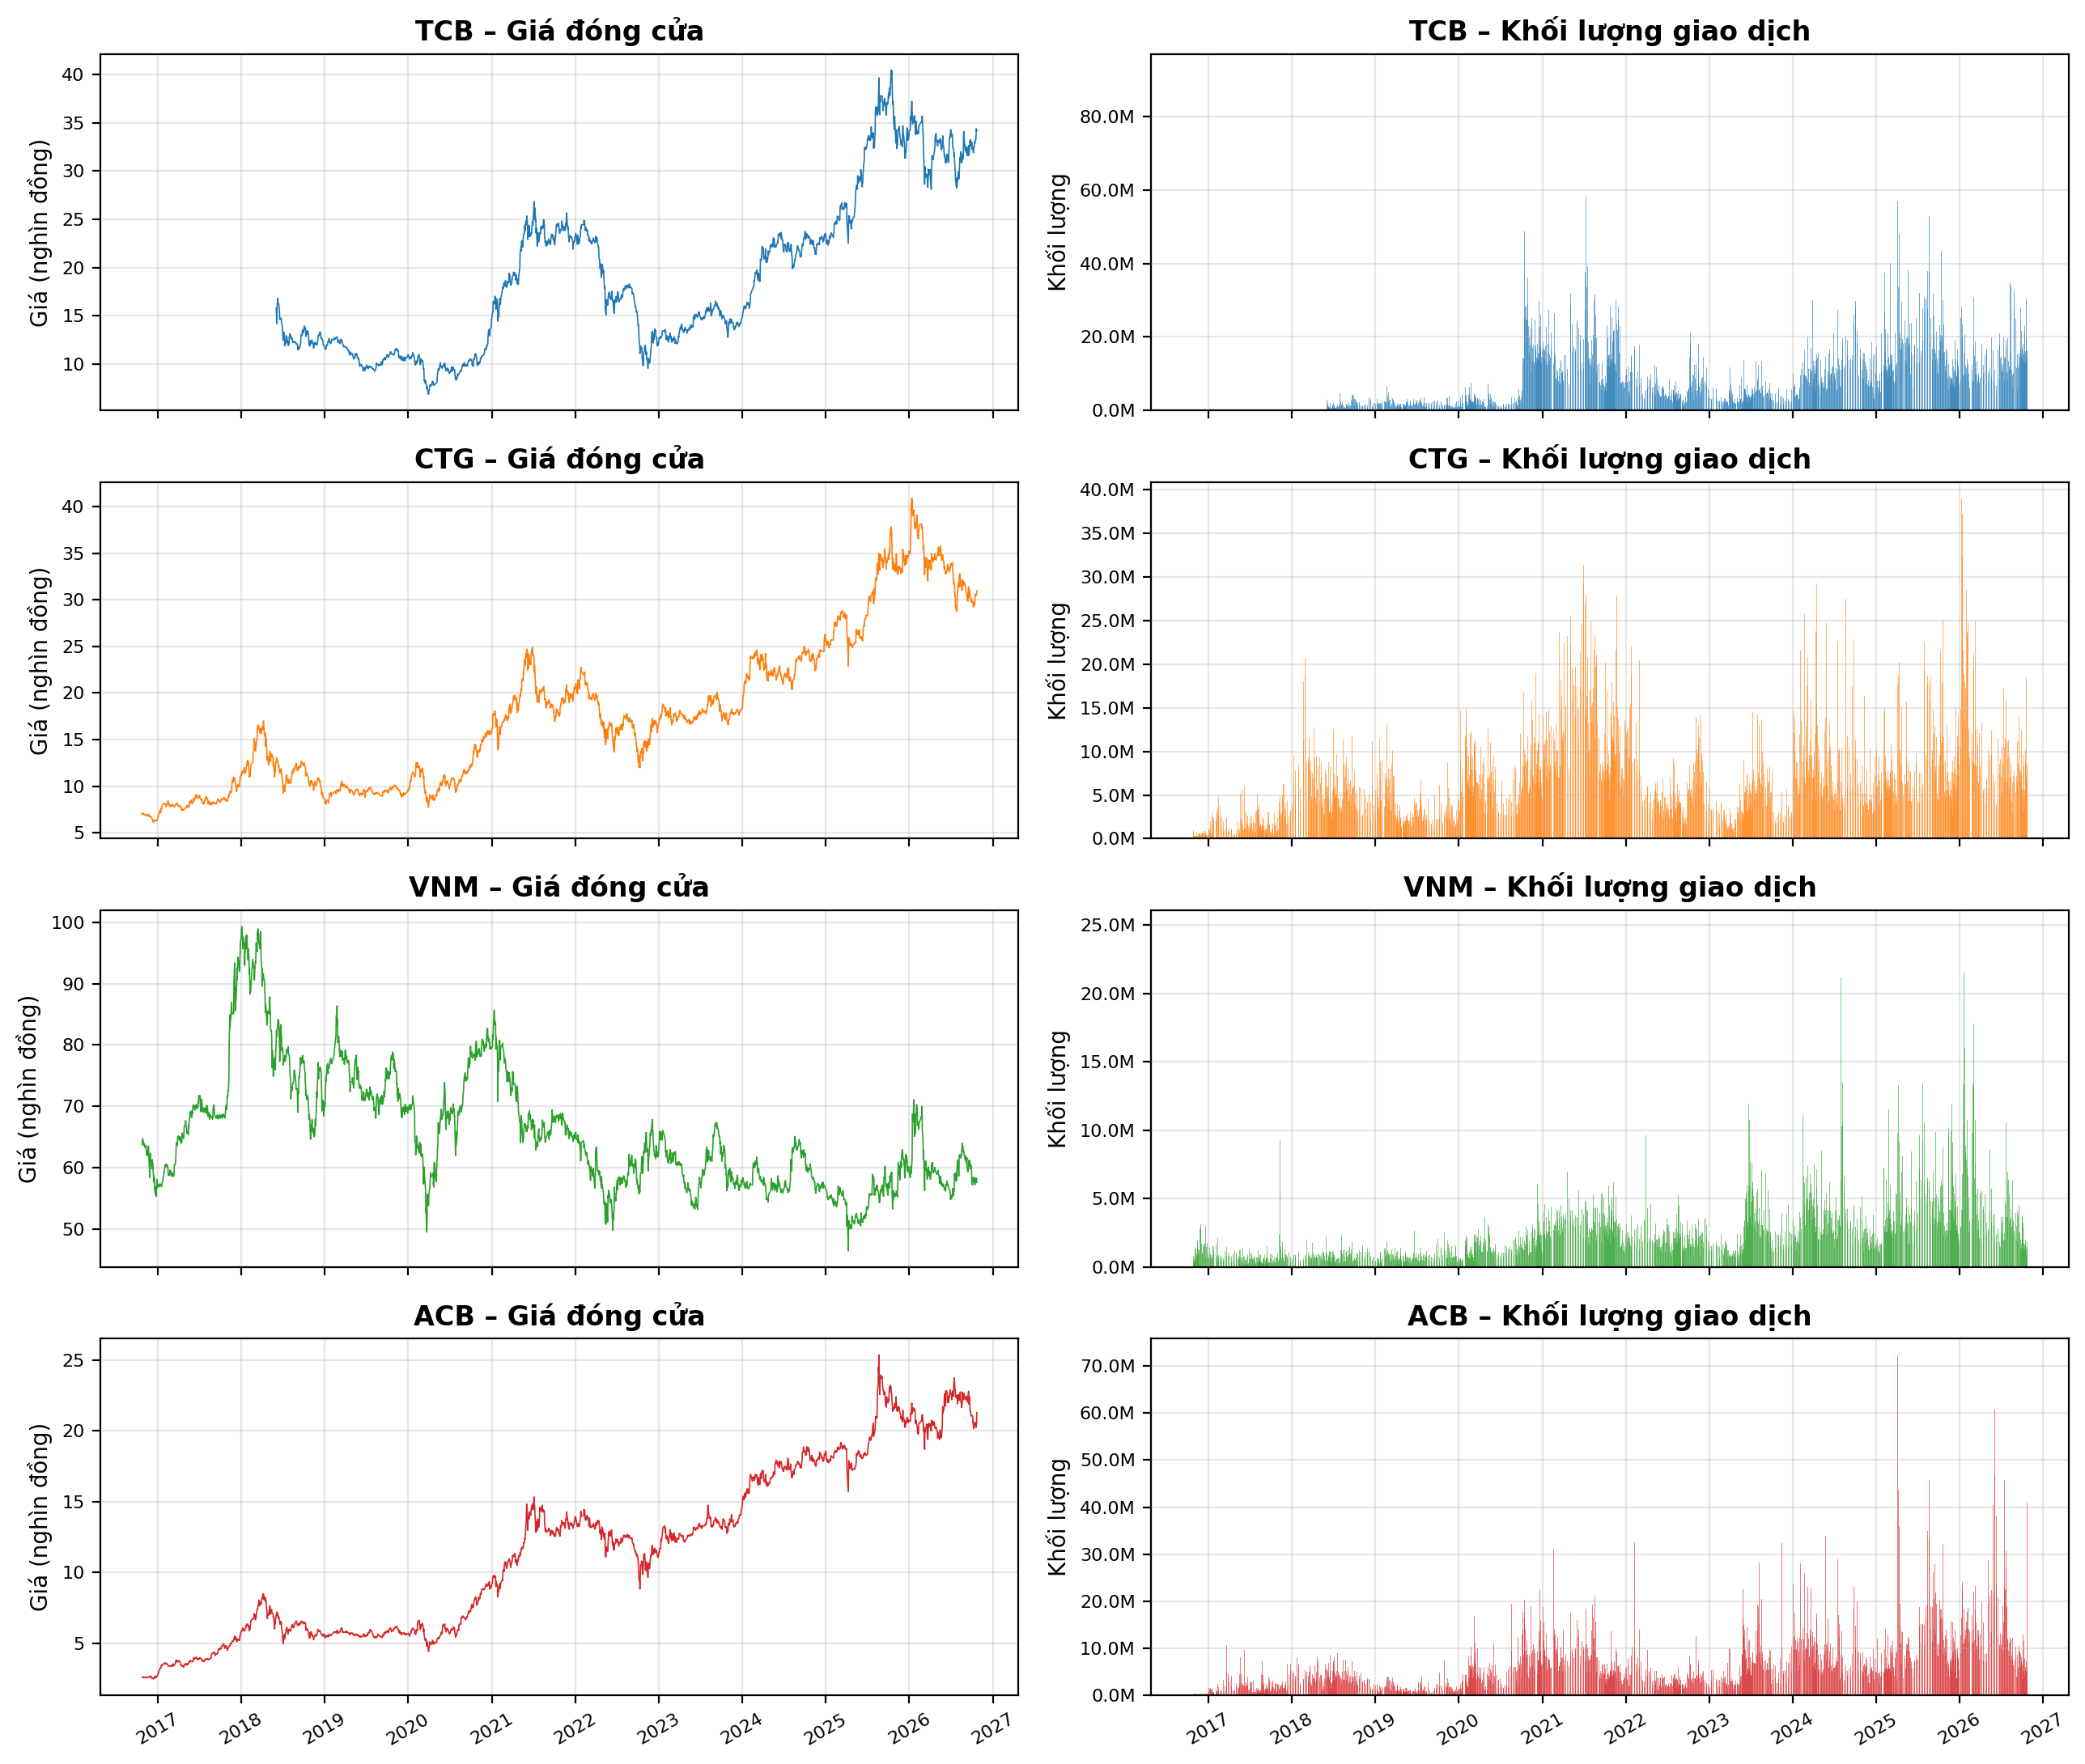
\includegraphics[width=0.80\textwidth]{close_volume.png}
  \caption{Giá đóng cửa và khối lượng giao dịch ngày của bốn mã cổ phiếu}
  \label{fig:closevolume}
\end{figure}

\textit{Nhận xét:}
\begin{itemize}
  \item Ba cổ phiếu ngân hàng (TCB, CTG, ACB) có xu hướng tăng trưởng dài hạn
    rõ rệt từ năm 2017 đến cuối 2026, xen kẽ các chu kỳ điều chỉnh mạnh tương ứng
    với biến động kinh tế vĩ mô: đợt bán tháo do đại dịch COVID-19 (quý 1/2020) và
    giai đoạn thắt chặt tín dụng, thanh lọc thị trường trái phiếu doanh nghiệp (nửa
    cuối 2022). Ngược lại, cổ phiếu tiêu dùng VNM duy trì xu hướng đi ngang và giảm
    nhẹ sau vùng đỉnh năm 2018.
  \item Khối lượng giao dịch có xu hướng gia tăng đột biến tại các vùng đáy điều
    chỉnh và các giai đoạn thị trường đảo chiều (hiện tượng cao trào khối lượng --
    \textit{volume climax}), phản ánh dòng tiền bắt đáy hoặc phân phối mạnh.
  \item Tính chất phi dừng (non-stationarity) rõ rệt của giá đóng cửa (trung bình
    và phương sai thay đổi liên tục theo thời gian) khẳng định tính đúng đắn của
    nguyên tắc thiết kế: \textbf{không đưa chuỗi giá thô vào mô hình học máy}, mà
    chuyển hóa thành các tỷ số so với đường trung bình và các chỉ báo kỹ thuật dừng.
\end{itemize}

\subsection{Phân bố lợi suất ngày}
Hình~\ref{fig:returndist} minh họa phân bố tần suất và hàm mật độ của lợi suất
logarit ngày $r_t = \ln(C_t / C_{t-1})$ cho từng mã.

\begin{figure}[H]
  \centering
  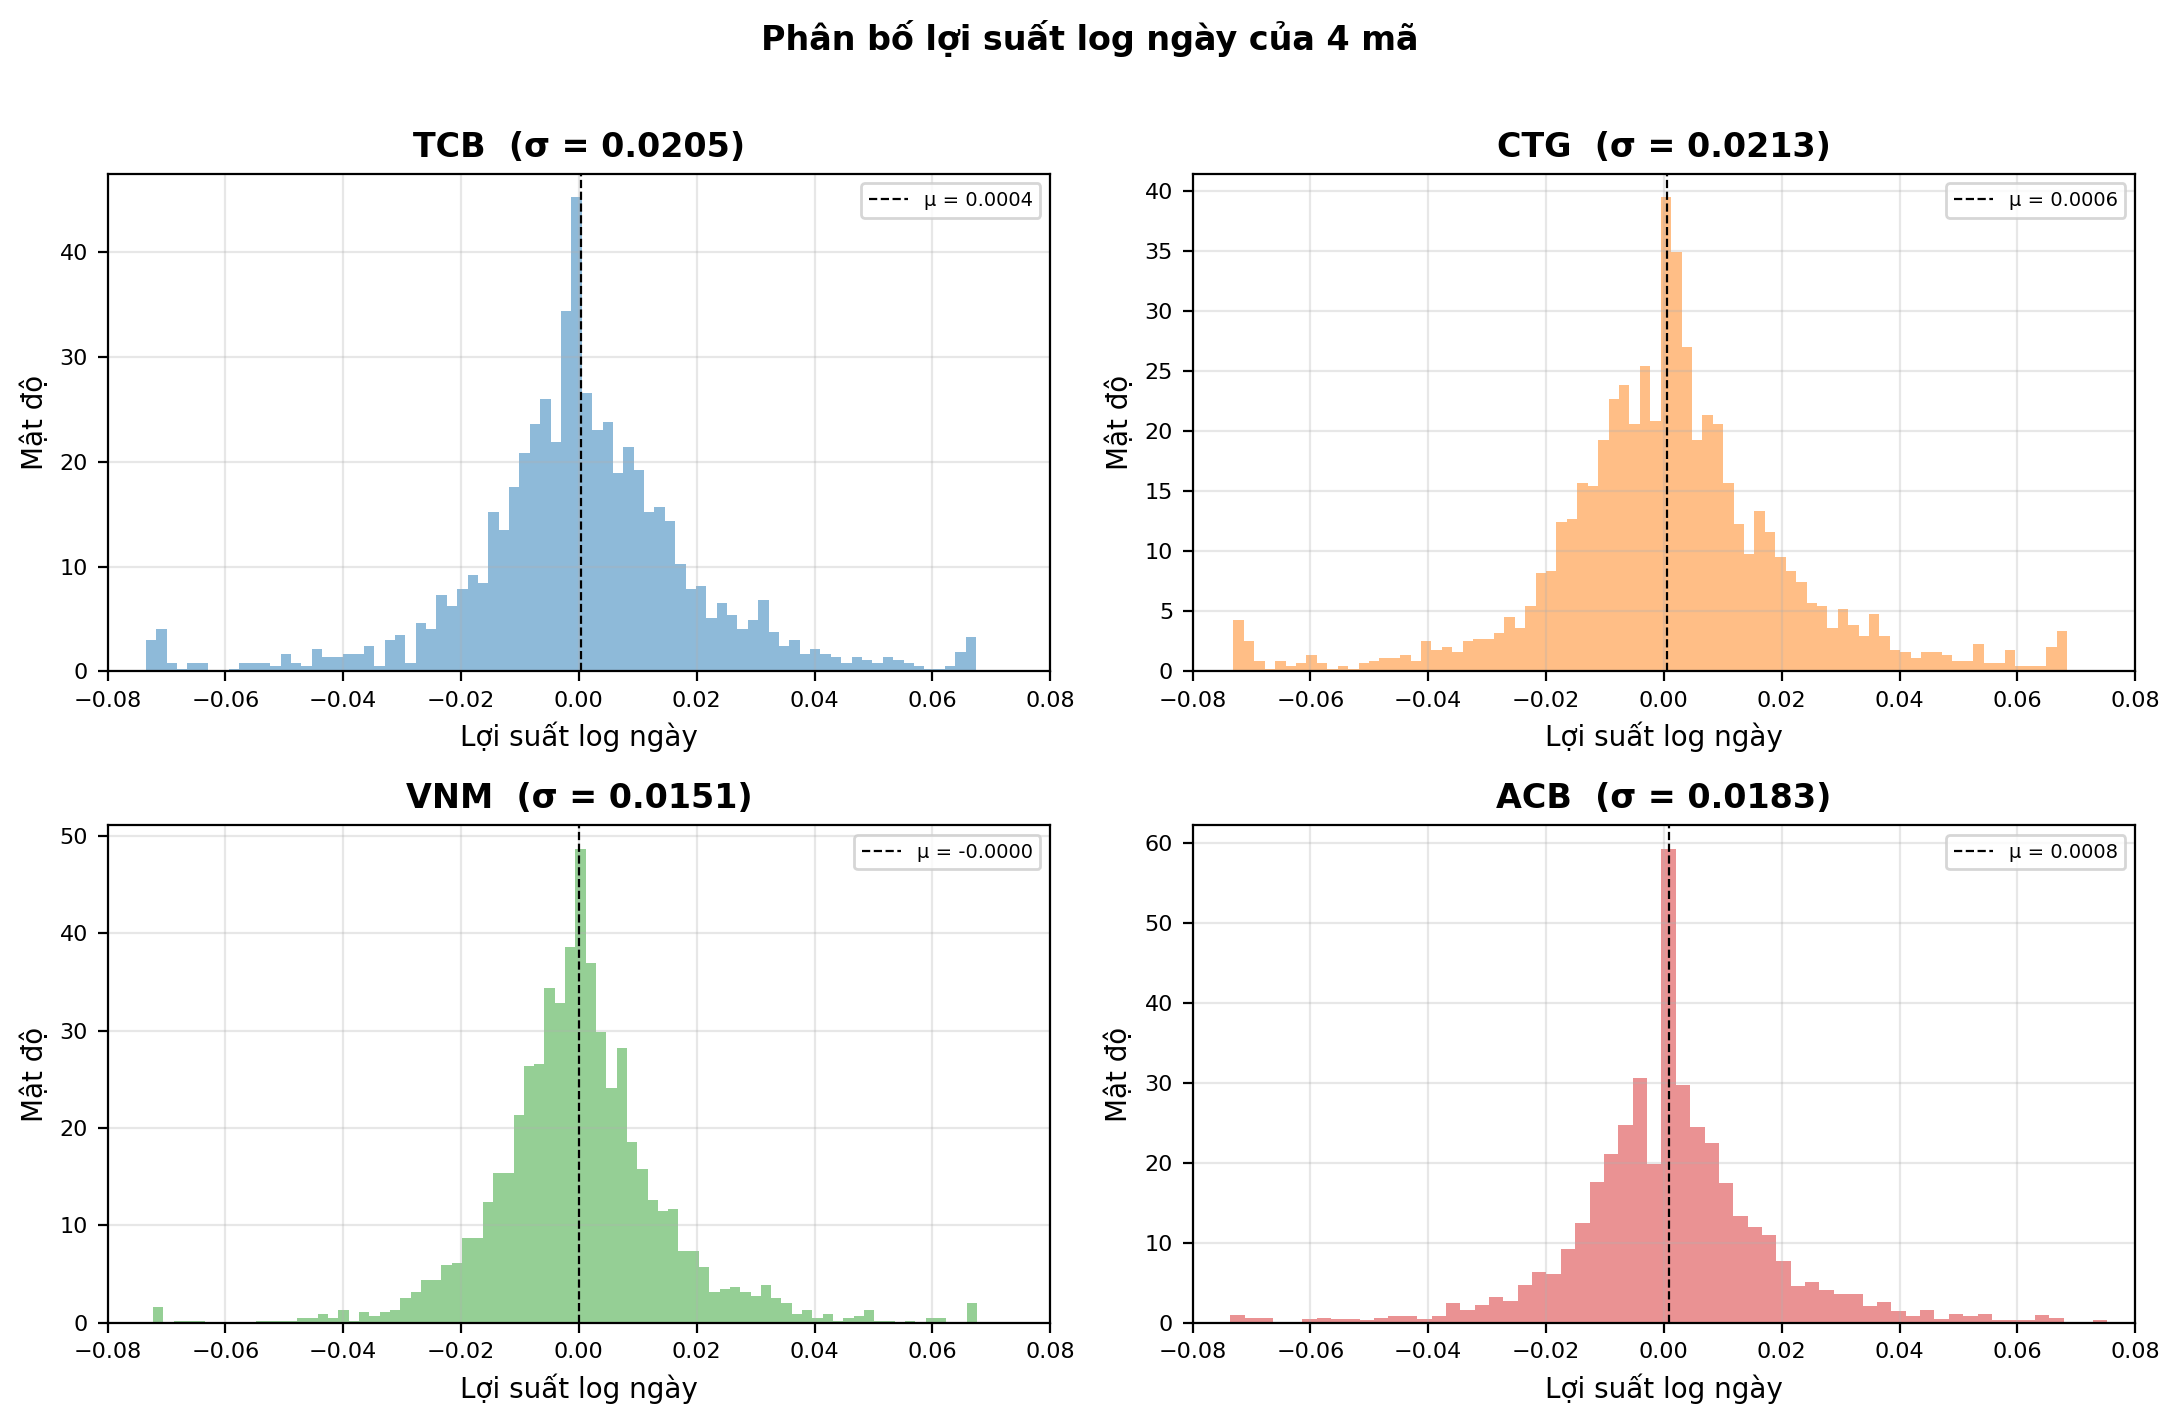
\includegraphics[width=0.80\textwidth]{return_dist.png}
  \caption{Phân bố tần suất lợi suất logarit ngày của bốn mã}
  \label{fig:returndist}
\end{figure}

\textit{Nhận xét:}
\begin{itemize}
  \item Lợi suất ngày của cả bốn mã phân bố gần đối xứng quanh giá trị trung bình
    xấp xỉ 0 ($\mu \in [0{,}0003;\, 0{,}0007]$), nhưng có dạng nhọn ở đỉnh và đuôi
    dày (leptokurtic) rõ rệt so với phân phối chuẩn Gauss. Hiện tượng này đặc trưng
    cho dữ liệu tài chính với tần suất xuất hiện các phiên biến động lớn cao hơn lý
    thuyết xác suất cổ điển.
  \item Độ lệch chuẩn lợi suất ngày $\sigma$ dao động từ $1{,}54\%$ (VNM) đến
    $2{,}08\%$ (TCB), phản ánh mức độ rủi ro và biên độ dao động của nhóm ngân hàng
    cao hơn đáng kể so với nhóm hàng tiêu dùng thiết yếu.
  \item Ngưỡng phân lớp $\theta = 0{,}5\%$ tương ứng với khoảng $0{,}25\sigma$ đến
    $0{,}33\sigma$, nằm vừa vặn trong vùng biến động thường nhật và tương đương với
    chi phí giao dịch thực tế (thuế $0{,}1\%$ + phí môi giới hai chiều $0{,}3\%$).
\end{itemize}

\subsection{Phân bố nhãn xu hướng}
Hình~\ref{fig:phanbonhan} thống kê số lượng và tỷ lệ phần trăm của ba lớp nhãn
(giảm: $-1$, ngang: $0$, tăng: $1$) với ngưỡng $\theta = 0{,}5\%$ trên tập dữ liệu
đã tiền xử lý.

\begin{figure}[H]
  \centering
  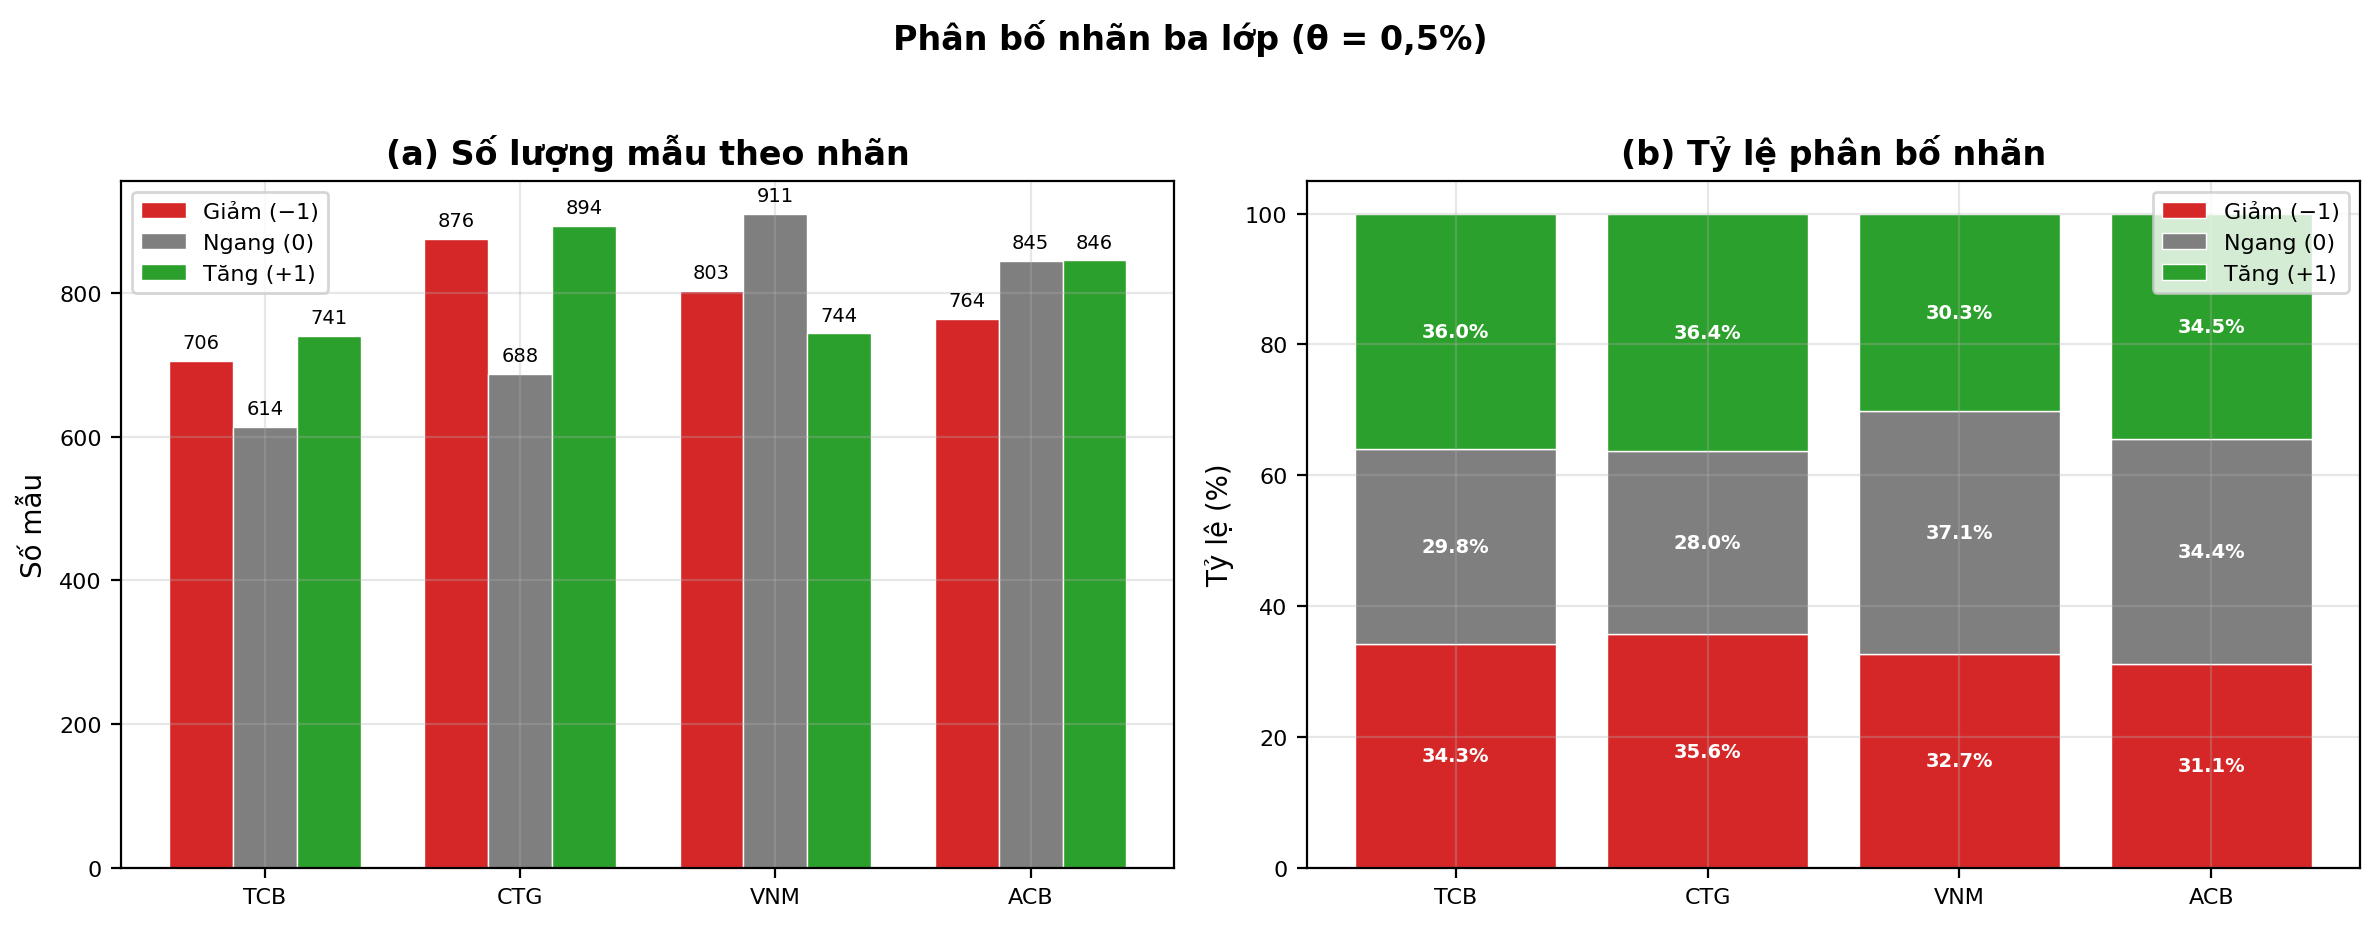
\includegraphics[width=0.82\textwidth]{label_dist.png}
  \caption{Số lượng và tỷ lệ phân bố ba lớp nhãn ($\theta = 0{,}5\%$) sau tiền xử lý}
  \label{fig:phanbonhan}
\end{figure}

\textit{Nhận xét:}
\begin{itemize}
  \item Tỷ lệ ba lớp tương đối cân bằng trên cả bốn mã: lớp giảm chiếm
    $31{,}1\%\text{--}35{,}6\%$, lớp ngang chiếm $28{,}0\%\text{--}37{,}1\%$, và
    lớp tăng chiếm $30{,}3\%\text{--}36{,}4\%$. Do độ lệch giữa các lớp không vượt
    quá $40\%$, tập dữ liệu không cần áp dụng các kỹ thuật cân bằng nhân tạo như
    SMOTE hay Random Undersampling (tránh nguy cơ bóp méo phân phối thời gian).
  \item Mã VNM có tỷ lệ phiên đi ngang cao nhất ($37{,}1\%$), phù hợp với độ biến
    động thấp đã quan sát ở phân bố lợi suất. Các mã tăng trưởng mạnh như TCB và
    CTG có tỷ lệ lớp tăng chiếm ưu thế ($36{,}0\%$ và $36{,}4\%$).
  \item Để đánh giá khách quan hiệu năng trên bài toán ba lớp gần cân bằng này,
    nhóm lựa chọn F1 macro và ROC-AUC macro làm các thước đo chất lượng chính thay
    vì chỉ dùng Accuracy.
\end{itemize}

\subsection{Tự tương quan của chuỗi lợi suất}
Hình~\ref{fig:autocorr} biểu diễn hệ số tự tương quan (Autocorrelation Function --
ACF) của chuỗi lợi suất ngày từ độ trễ 1 đến 20 phiên.

\begin{figure}[H]
  \centering
  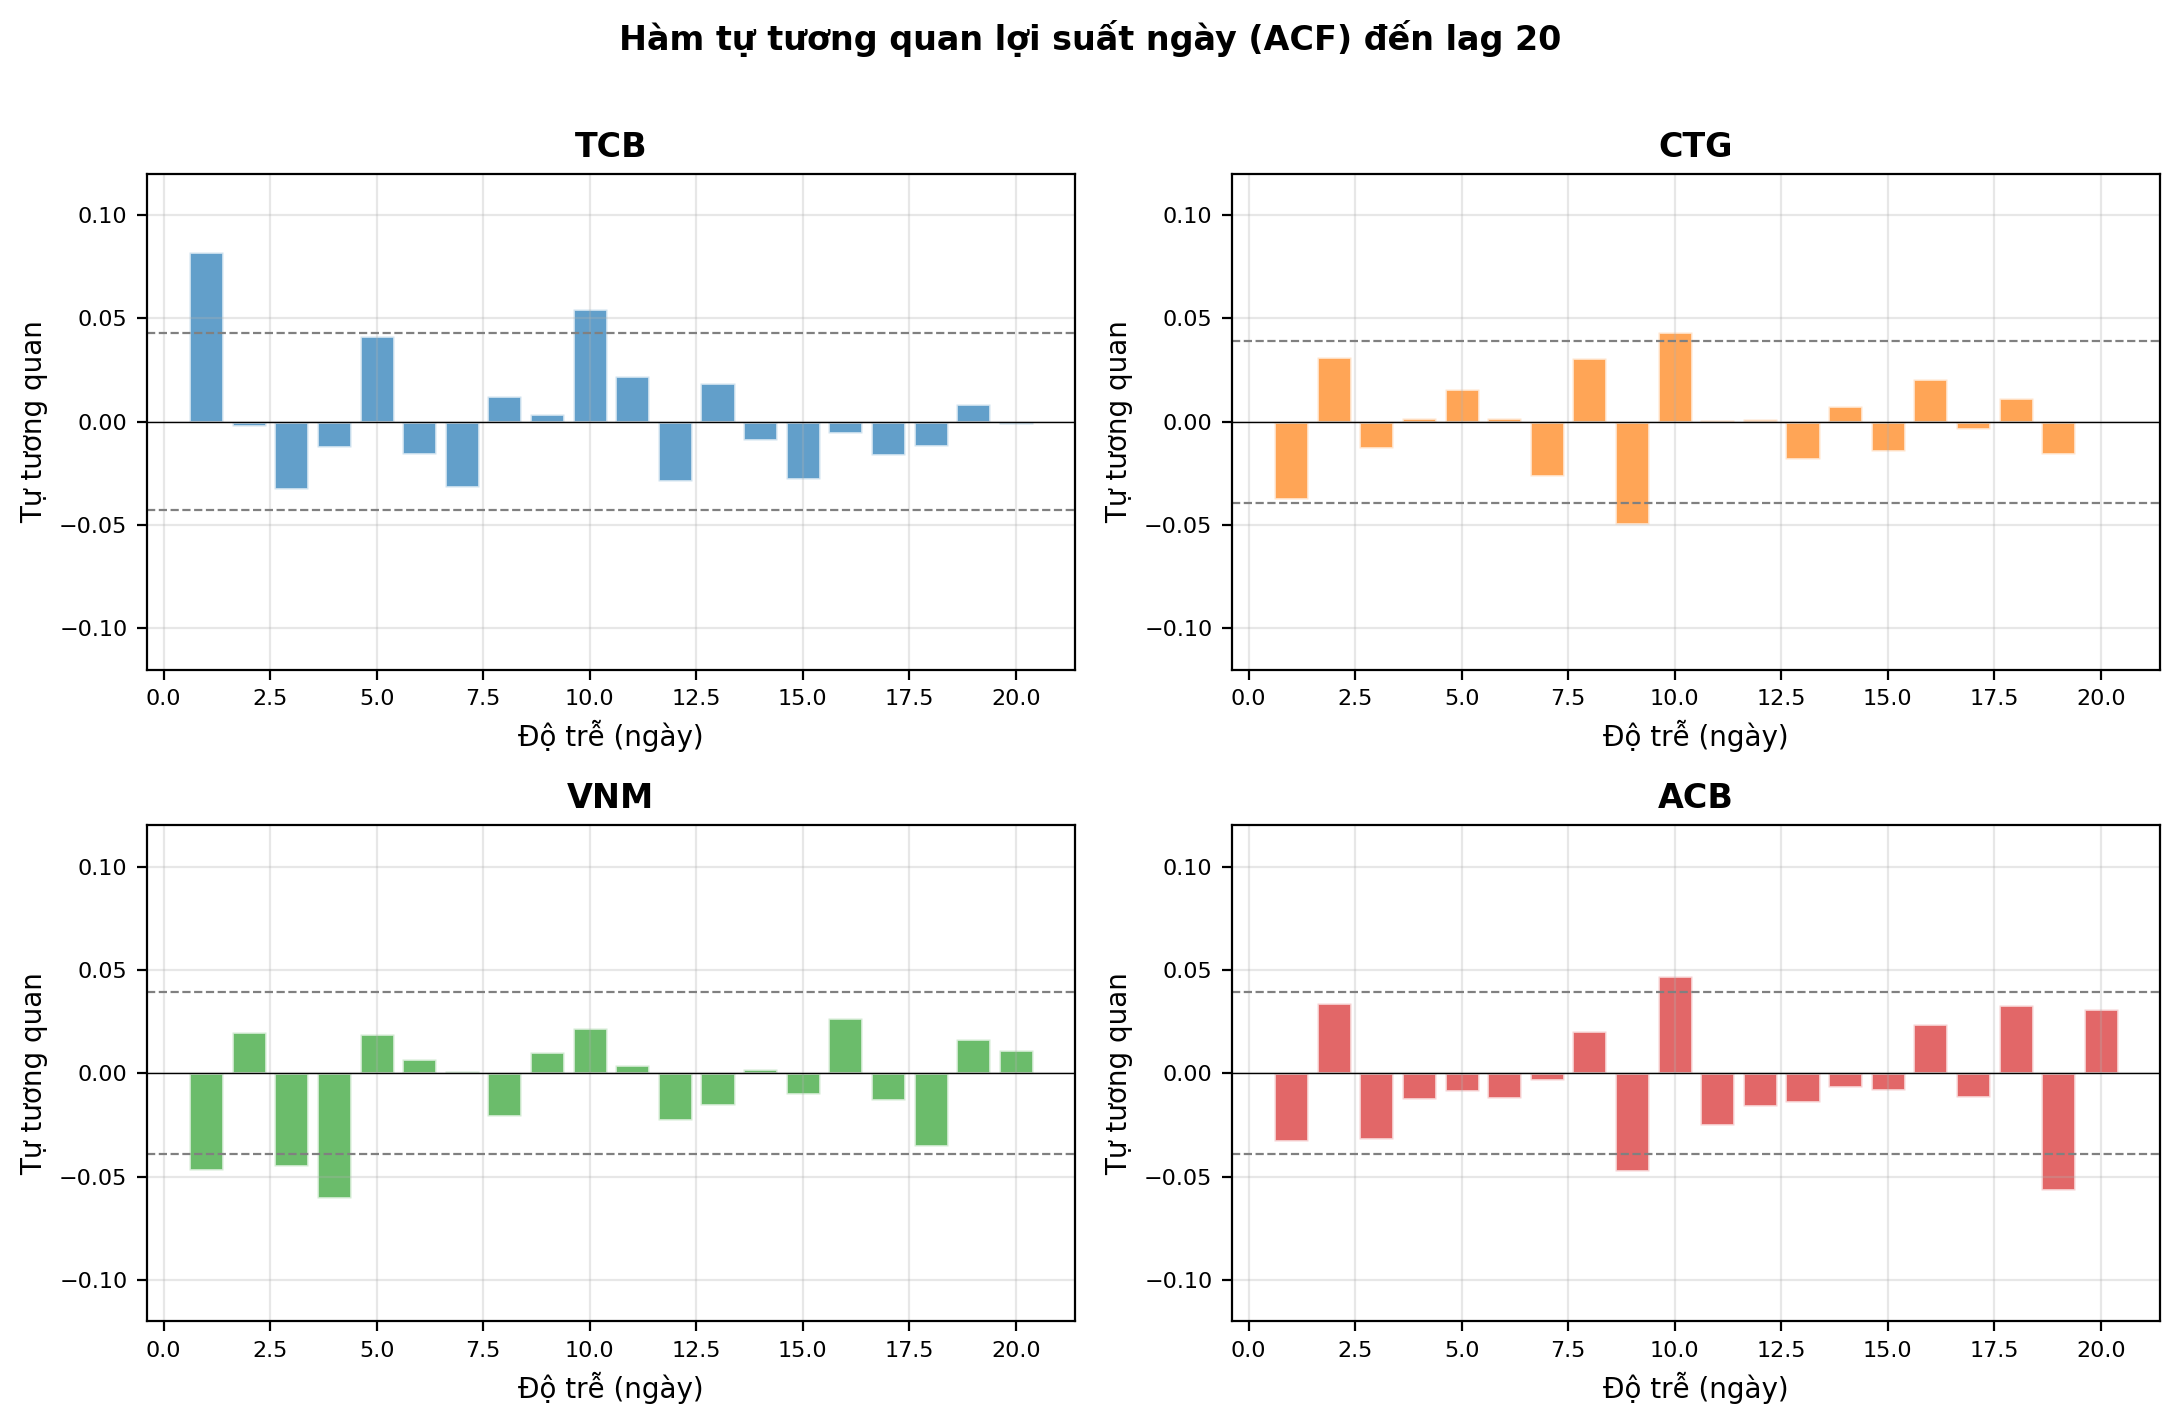
\includegraphics[width=0.80\textwidth]{autocorr.png}
  \caption{Hàm tự tương quan (ACF) của lợi suất ngày đến lag 20 kèm dải tin cậy 95\%}
  \label{fig:autocorr}
\end{figure}

\textit{Nhận xét:}
\begin{itemize}
  \item Hệ số tự tương quan tại hầu hết các độ trễ đều rất nhỏ ($|r| < 0{,}05$) và
    nằm hoàn toàn bên trong dải tin cậy 95\% ($\pm 1{,}96/\sqrt{n}$, biểu thị bằng
    đường nét đứt xám).
  \item Kết quả này hoàn toàn nhất quán với Giả thuyết thị trường hiệu quả dạng yếu
    (Weak-form EMH) của Fama~\cite{fama1970}: lợi suất phiên kế tiếp không có quan
    hệ tuyến tính trực tiếp với lợi suất các phiên quá khứ gần nhất.
  \item Điều đó giải thích vì sao các mô hình tuyến tính đơn giản chỉ dùng độ trễ
    giá thường thất bại, và đặt ra sự cần thiết phải tích hợp các chỉ báo động lượng,
    xu hướng và biến động phi tuyến, cùng các thuật toán phi tuyến tính như Rừng
    ngẫu nhiên và XGBoost.
\end{itemize}

\subsection{Quan hệ tương quan giữa các đặc trưng}
Hình~\ref{fig:tuongquan} trình bày ma trận tương quan Pearson giữa 25 đặc trưng sau
khi chuẩn hóa, được tính toán trên toàn bộ dữ liệu gộp của bốn mã cổ phiếu.

\begin{figure}[H]
  \centering
  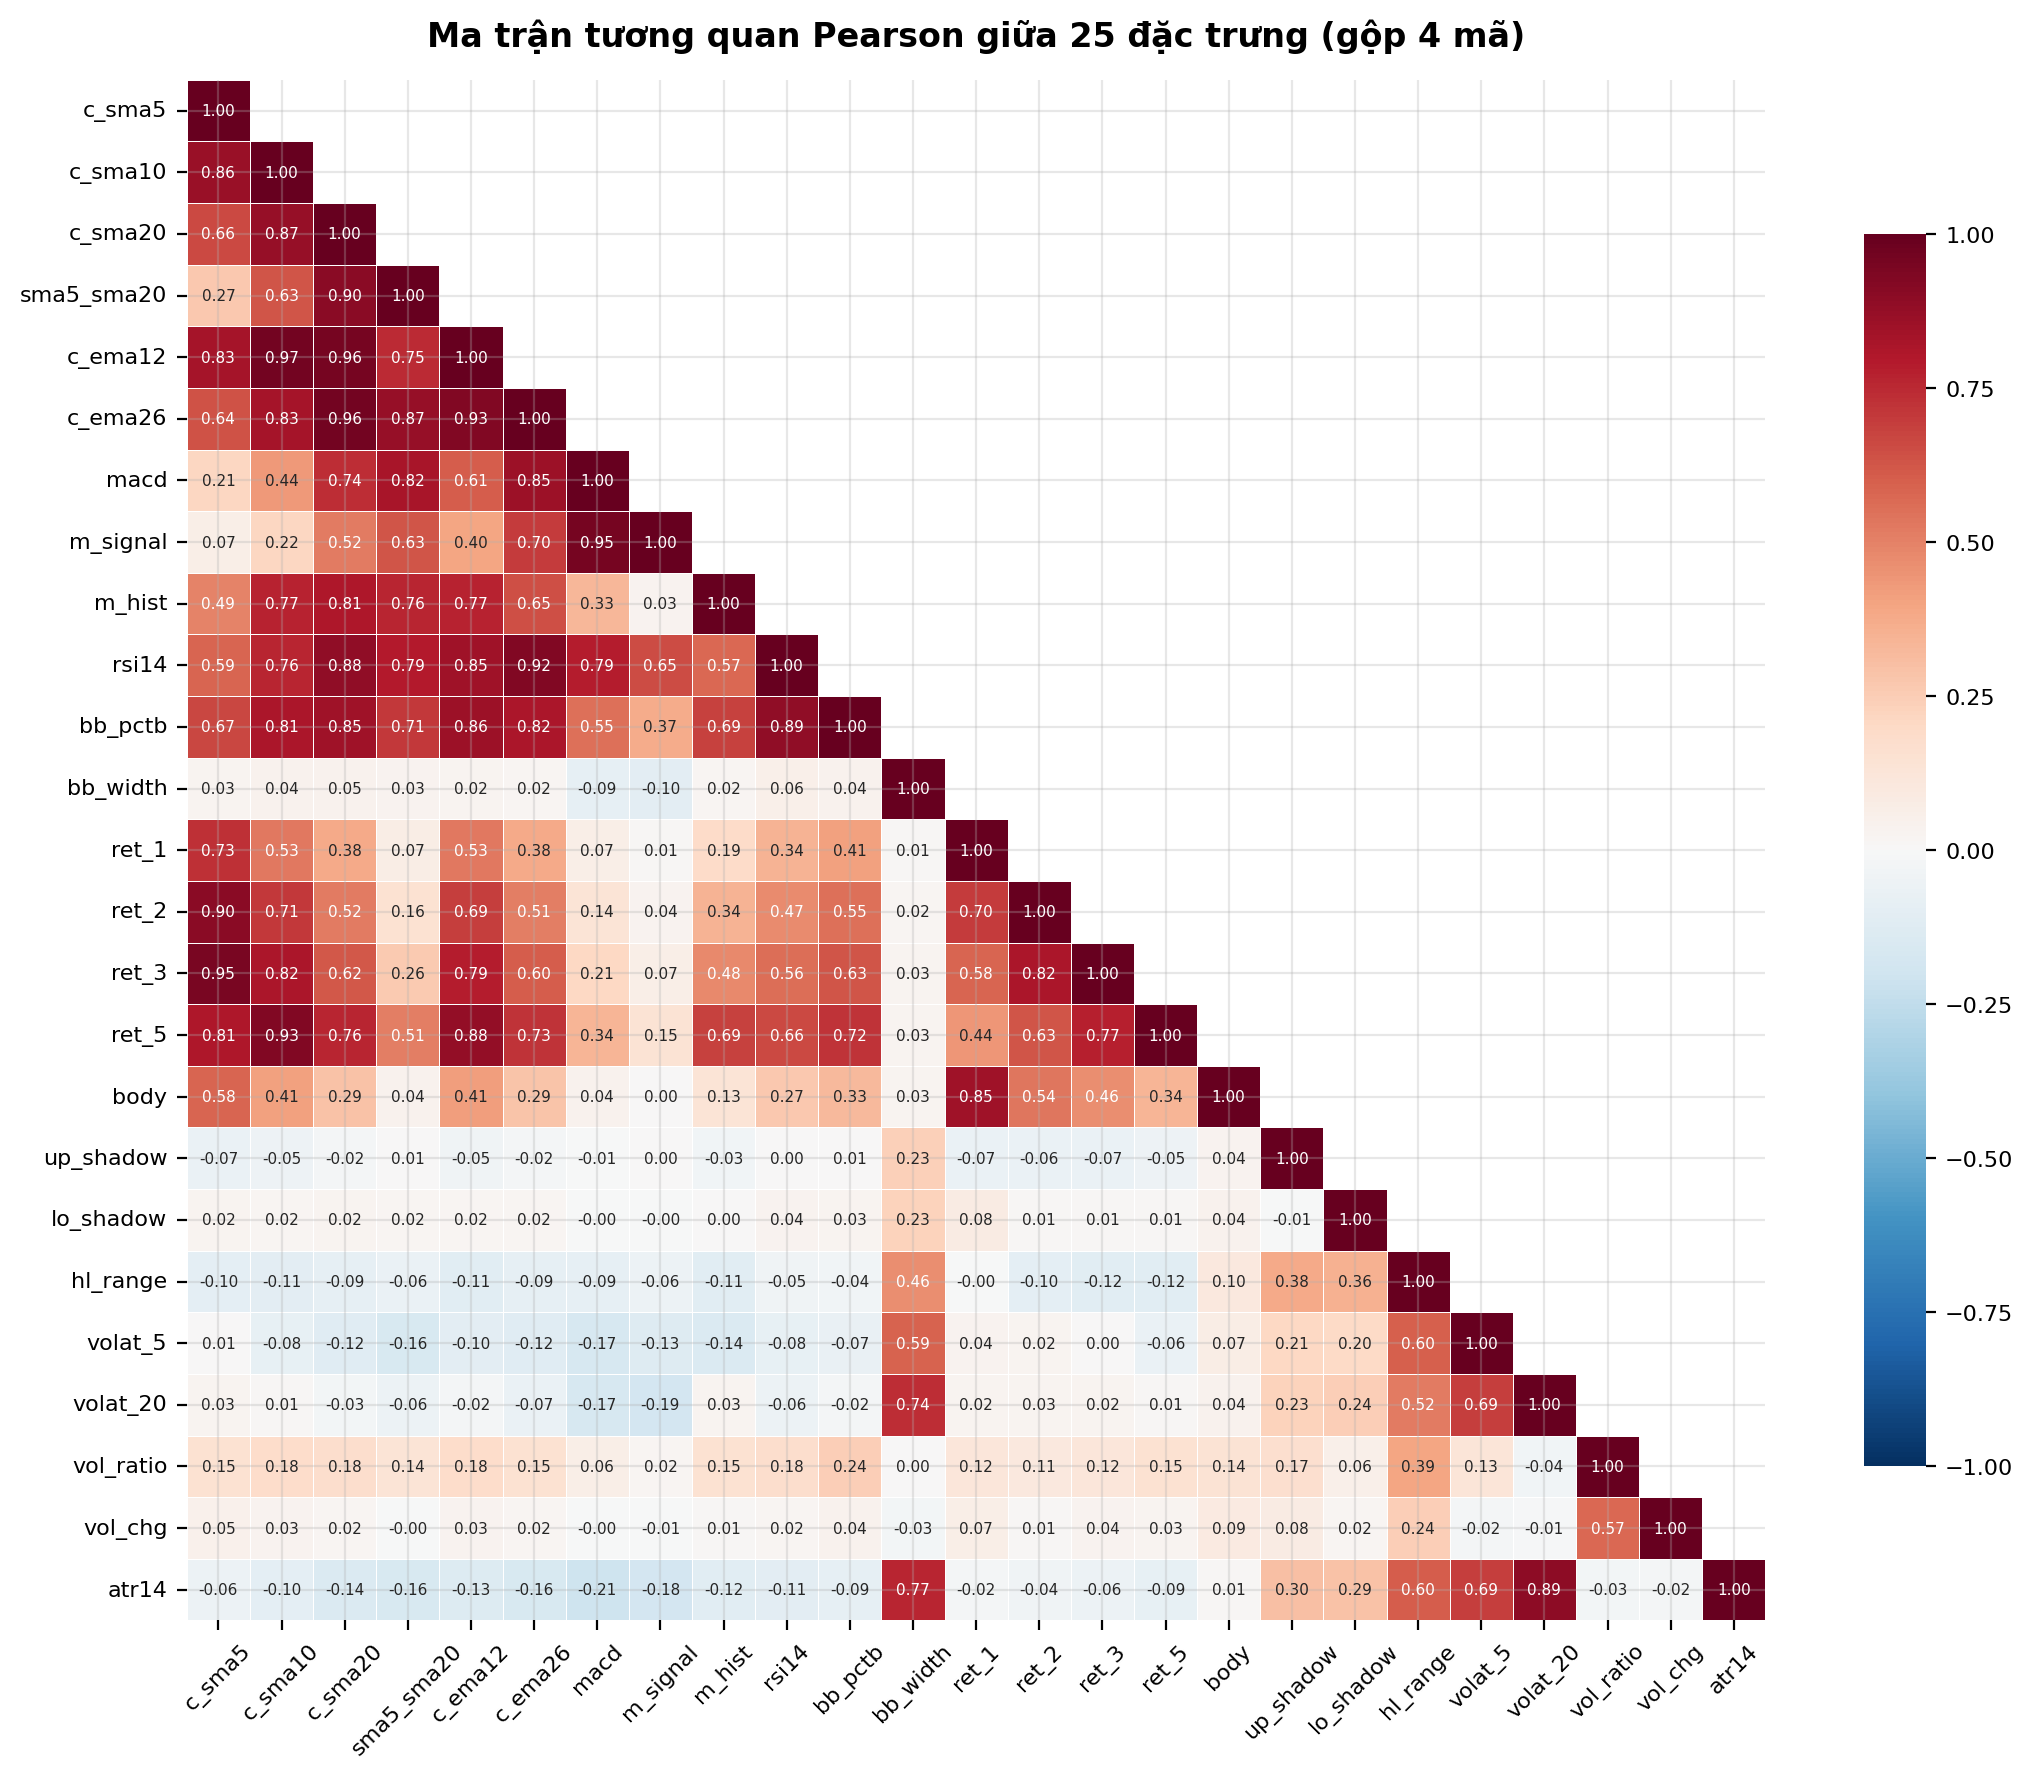
\includegraphics[width=0.72\textwidth]{corr_matrix.png}
  \caption{Ma trận tương quan Pearson giữa 25 đặc trưng số (gộp 4 mã)}
  \label{fig:tuongquan}
\end{figure}

\textit{Nhận xét:}
\begin{enumerate}
  \item \textbf{Cụm đặc trưng xu hướng và vị thế giá:} Các đặc trưng đo khoảng cách
    giữa giá đóng cửa và các đường trung bình động (\texttt{close\_sma5},
    \texttt{close\_sma10}, \texttt{close\_sma20}, \texttt{close\_ema12},
    \texttt{close\_ema26}) có hệ số tương quan thuận rất cao ($r > 0{,}80$). Đặc
    biệt, \texttt{bb\_pctb} (vị trí tương đối trong dải Bollinger) có tương quan lên
    tới $0{,}95$ với \texttt{close\_sma20} do cùng sử dụng trung bình động 20 phiên
    làm trục cơ sở.
  \item \textbf{Cụm đặc trưng độ biến động:} \texttt{volat\_5}, \texttt{volat\_20},
    \texttt{hl\_range}, \texttt{bb\_width} và \texttt{atr14} tạo thành một nhóm có
    tương quan dương rõ rệt ($r \in [0{,}55;\, 0{,}85]$), cùng phản ánh trạng thái
    dao động mạnh hay hẹp của thị trường trong phiên.
  \item \textbf{Tính độc lập của tín hiệu khối lượng:} Các đặc trưng liên quan đến
    khối lượng (\texttt{vol\_ratio}, \texttt{vol\_chg}) có mức độ tương quan tuyến
    tính rất thấp với các đặc trưng giá và biến động ($|r| < 0{,}15$), chứng minh
    khối lượng mang lại nguồn thông tin bổ trợ trực giao, không bị trùng lặp với
    hành động giá.
  \item \textbf{Ý nghĩa với mô hình hóa:} Hiện tượng đa cộng tuyến giữa các chỉ báo
    xu hướng đòi hỏi Hồi quy Logistic phải sử dụng chuẩn hóa $L_2$ (Ridge penalty)
    để ổn định trọng số; trong khi các thuật toán cây như Rừng ngẫu nhiên và XGBoost
    vốn có cơ chế chọn ngẫu nhiên tập con đặc trưng (feature subsampling) nên sẽ ít
    bị tổn hại bởi hiện tượng này.
\end{enumerate}

\subsection{Phân bố các đặc trưng chính theo nhãn xu hướng}
Hình~\ref{fig:featlabel} trình bày biểu đồ hộp (boxplot) của sáu đặc trưng đại diện
cho ba nhóm (lợi suất, động lượng, biến động) phân theo ba lớp nhãn $-1$, $0$ và $1$.

\begin{figure}[H]
  \centering
  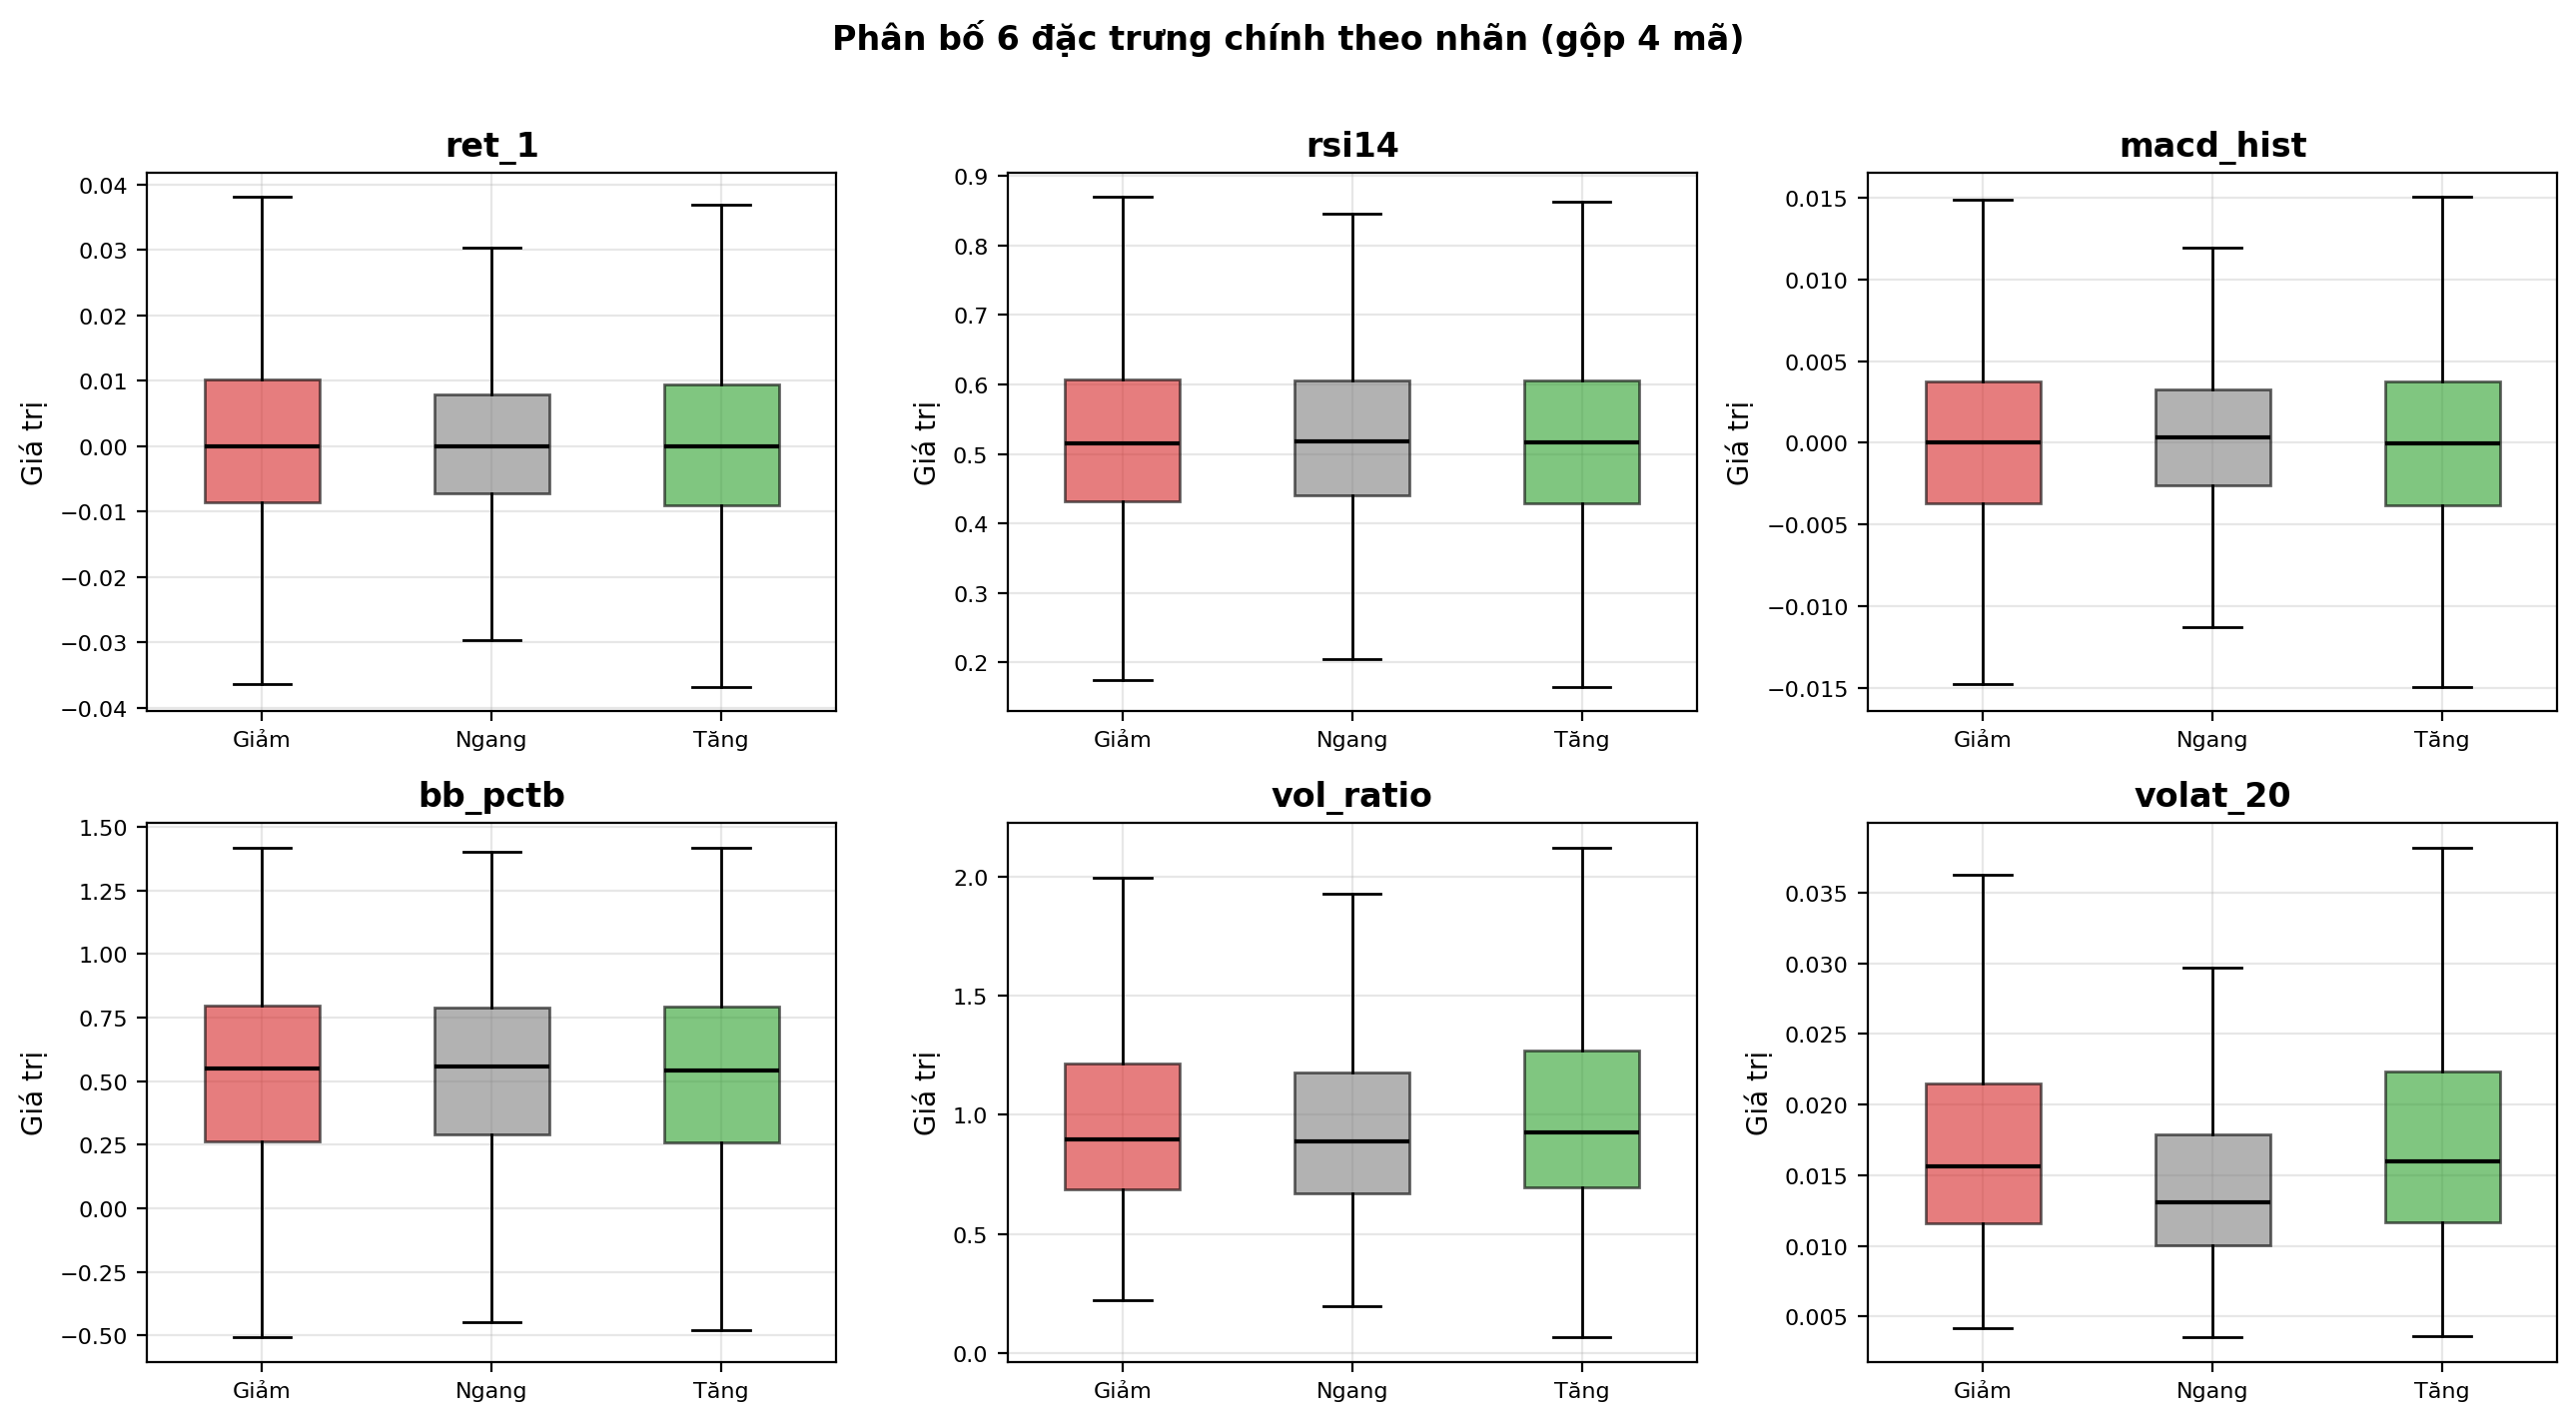
\includegraphics[width=0.80\textwidth]{features_by_label.png}
  \caption{Phân bố 6 đặc trưng đại diện theo ba lớp nhãn xu hướng (gộp 4 mã)}
  \label{fig:featlabel}
\end{figure}

\textit{Nhận xét:}
\begin{itemize}
  \item \texttt{ret\_1} thể hiện sự dịch chuyển trung vị rõ nét nhất giữa các lớp:
    phiên trước tăng thường đi kèm với xu hướng phân loại nhất định, tuy nhiên khoảng
    tứ phân vị (IQR) giữa ba lớp vẫn chồng lấn đáng kể, khẳng định bài toán có độ
    nhiễu cao và không thể phân loại bằng một ranh giới đơn biến tầm thường.
  \item Chỉ báo động lượng \texttt{rsi14} và \texttt{macd\_hist} có phân bố lệch
    nhẹ sang giá trị cao hơn ở lớp tăng ($1$) và thấp hơn ở lớp giảm ($-1$), thể hiện
    tín hiệu động lượng có giá trị dự báo nhưng cần được kết hợp với các bộ lọc phụ trợ.
  \item Các đặc trưng biến động (\texttt{volat\_20}) và khối lượng (\texttt{vol\_ratio})
    có hình dạng phân phối tương đồng giữa ba nhãn; vai trò của chúng trong mô hình
    không phải là yếu tố phân tách tuyến tính trực tiếp mà là các điều kiện kích hoạt
    phi tuyến trong cây quyết định (ví dụ: chỉ báo RSI hiệu quả hơn trong môi trường
    biến động thấp).
\end{itemize}

\section{Phát hiện và xử lý vấn đề chất lượng dữ liệu}
\label{sec:chatluong}

Bảng~\ref{tab:chatluong} tổng hợp các vấn đề đã kiểm tra trên dữ liệu thô của
bốn mã và cách xử lý đã được cài đặt trong \texttt{clean\_data.py}.

\begin{longtable}{p{2.9cm} >{\centering\arraybackslash}p{3.4cm} p{8.6cm}}
  \caption{Thống kê các vấn đề chất lượng dữ liệu và cách xử lý}\label{tab:chatluong}\\
  \toprule
  \textbf{Vấn đề} & \textbf{Số lượng (tỷ lệ)} & \textbf{Cách xử lý và lý do} \\
  \midrule
  \endfirsthead
  \toprule
  \textbf{Vấn đề} & \textbf{Số lượng (tỷ lệ)} & \textbf{Cách xử lý và lý do} \\
  \midrule
  \endhead
  \bottomrule
  \endfoot
        Giá trị thiếu & 0 & Không cần xử lý. Nếu xuất hiện thì bỏ dòng, không nội suy vì giá là dữ liệu quan sát thực \\
    Khối lượng bằng 0 & 0 & Nếu có thì bỏ dòng (ngày không giao dịch) \\
    Bản ghi trùng ngày & 1 ngày (27/12/2022) tách thành 2 nến ở cả 4 mã & Gộp: \texttt{open} của nến đầu, \texttt{high} lớn nhất, \texttt{low} nhỏ nhất, \texttt{close} của nến cuối, \texttt{volume} cộng dồn. Đây là lỗi nguồn nên giữ cả hai nến sẽ tạo lợi suất sai \\
    OHLC sai logic (\texttt{open}/\texttt{close} ngoài $[\texttt{low},\texttt{high}]$) & 3 nến: TCB 18/07/2019; VNM 15/07/2019 và 30/08/2019 & Kẹp lại \texttt{high} $=\max(o,h,c)$, \texttt{low} $=\min(o,l,c)$ để giữ nguyên số nến \\
    Biến động bất thường & ACB có 12 phiên $>7{,}5\%$ đến 06/2020 & Giữ nguyên: đều nằm trong biên $\pm 10\%$ của HNX nên là biến động thật \\
    Nến chưa đóng & 0 (nến cuối là 23/10/2026) & Bỏ nến của ngày hiện tại nếu thu thập trước 15:00 \\
    Mất cân bằng lớp (giảm / ngang / tăng, $\theta = 0{,}5\%$) & TCB 706/614/741; CTG 876/688/894; VNM 803/911/744; ACB 764/845/846 & Ba lớp gần cân bằng nên không cần lấy mẫu lại; đánh giá bằng F1 macro và ROC-AUC macro thay vì chỉ Accuracy \\
    Nguy cơ rò rỉ dữ liệu & Hai cột nhìn về tương lai: \texttt{label}, \texttt{r\_next} & Không đưa vào đặc trưng; chia dữ liệu theo thời gian, bỏ 1 phiên giữa train và test, scaler chỉ fit trên tập train của từng fold \\
\end{longtable}

\begin{table}[H]
  \centering
  \caption{So sánh số nến trước và sau làm sạch dữ liệu 1D}
  \label{tab:truocsau}
  \begin{tabular}{lrrrr}
    \toprule
    \textbf{Mã} & \textbf{Trước} & \textbf{Gộp trùng} & \textbf{Sửa OHLC} & \textbf{Sau} \\
    \midrule
    TCB & 2\,098 & 1 & 1 & 2\,097 \\
    CTG & 2\,495 & 1 & 0 & 2\,494 \\
    VNM & 2\,495 & 1 & 2 & 2\,494 \\
    ACB & 2\,492 & 1 & 0 & 2\,491 \\
    \bottomrule
  \end{tabular}
\end{table}

Sau làm sạch, cả bốn tệp không còn giá trị thiếu, ngày trùng, volume không dương
hoặc nến vi phạm quan hệ OHLC. Các phiên biến động mạnh hợp lệ vẫn được giữ nguyên.

\section{Chuẩn bị dữ liệu cho mô hình}
Toàn bộ 25 đặc trưng đều là số nên không cần mã hóa biến phân loại; nhãn
$\{-1,0,1\}$ chỉ được ánh xạ thành $\{0,1,2\}$ khi huấn luyện XGBoost. Việc chuẩn
hóa chỉ áp dụng cho Hồi quy Logistic bằng \texttt{StandardScaler}, được khớp trên
tập huấn luyện của từng fold rồi áp dụng cho khối kiểm tra của fold đó; Rừng ngẫu
nhiên và XGBoost không cần chuẩn hóa. Dữ liệu không được xáo trộn mà chia theo thời
gian bằng walk-forward như ở Mục~\ref{sec:quytrinh}.

Hình~\ref{fig:walkforwardthucte} minh họa trực quan cấu trúc các fold kiểm định
walk-forward thực tế được tạo ra cho mã CTG (27 fold). Cơ chế cửa sổ mở rộng
(expanding window) giúp tập huấn luyện tích lũy dữ liệu lịch sử theo thời gian,
khối kiểm tra 63 phiên liền kề không chồng lấn, và khoảng cách ly (purge) 1 phiên
được duy trì nghiêm ngặt giữa tập huấn luyện và kiểm tra nhằm ngăn chặn việc nhãn
phiên cuối của tập train sử dụng giá đóng cửa phiên đầu của tập test.

\begin{figure}[H]
  \centering
  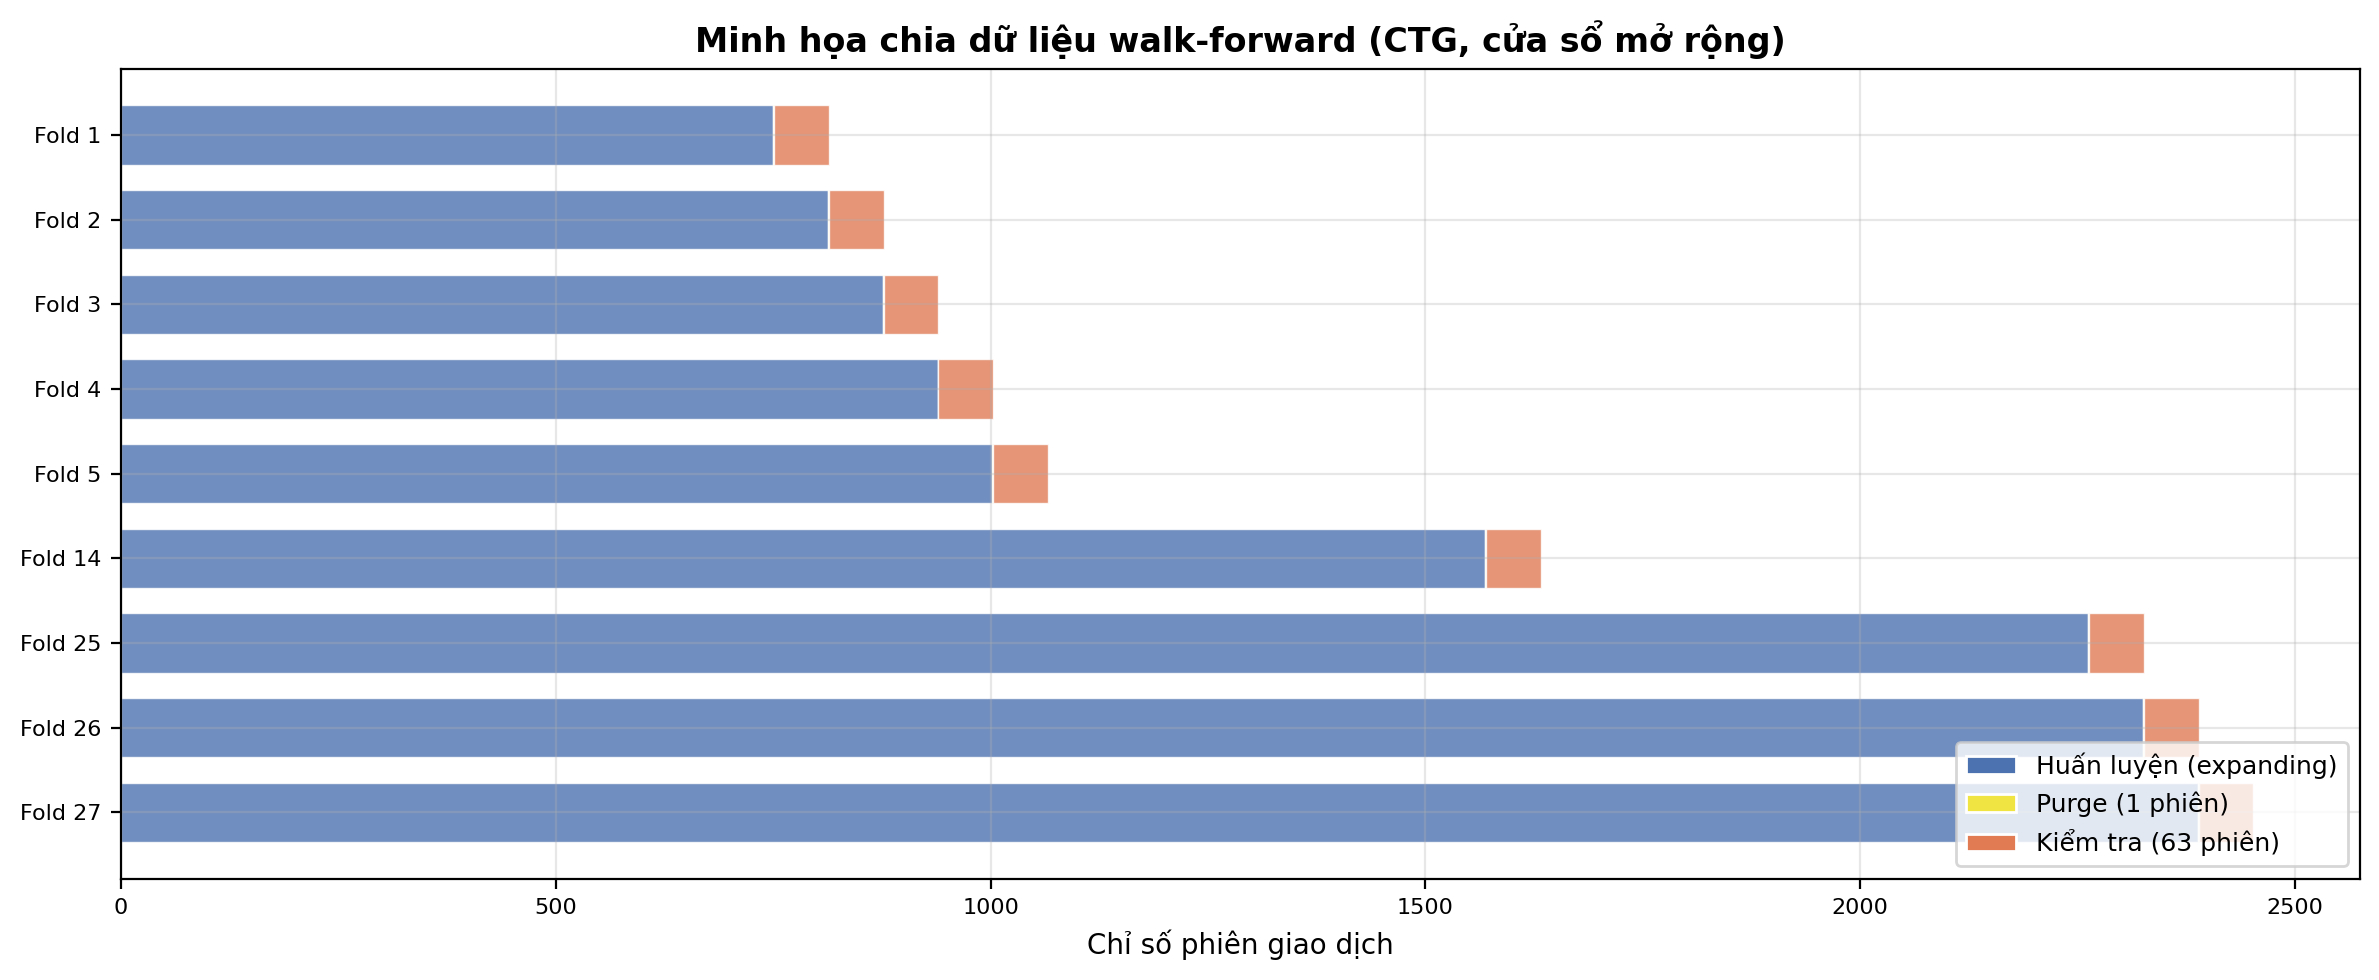
\includegraphics[width=0.85\textwidth]{walk_forward.png}
  \caption{Minh họa các fold kiểm định walk-forward thực tế trên mã CTG (27 fold)}
  \label{fig:walkforwardthucte}
\end{figure}

Sau khi bỏ 35 phiên khởi động (do chỉ báo dài nhất cần EMA26 rồi EMA9) và phiên cuối
không có nhãn, mã tiền xử lý tạo ra kích thước dữ liệu thực tế ở
Bảng~\ref{tab:kichthuoc}.

\begin{table}[H]
  \centering
  \caption{Kích thước dữ liệu đã tiền xử lý và số fold walk-forward}
  \label{tab:kichthuoc}
  \begin{tabular}{lccccc}
    \toprule
    \textbf{Mã} & \textbf{Số mẫu} & \textbf{Số đặc trưng} & \textbf{Train đầu} & \textbf{Test/fold} & \textbf{Số fold} \\
    \midrule
    TCB & 2\,061 & 25 & 750 & 63 & 20 \\
    CTG & 2\,458 & 25 & 750 & 63 & 27 \\
    VNM & 2\,458 & 25 & 750 & 63 & 27 \\
    ACB & 2\,455 & 25 & 750 & 63 & 27 \\
    \bottomrule
  \end{tabular}
\end{table}

Các tệp đầu ra bắt đầu từ 23/07/2018 đối với TCB và 14/12/2016 đối với ba mã
còn lại; ngày cuối có nhãn là 22/10/2026. Số liệu chi tiết và phân bố nhãn được
lưu tại \texttt{data/processed/1D/preprocessing\_summary.csv}.

Ngoài khung chính 1D, quy trình đã tạo dữ liệu sẵn sàng cho thí nghiệm ở năm
khung nội ngày. Ngưỡng nhãn được chọn theo độ biến động và bước giá thực tế
trước khi huấn luyện; mỗi khung vẫn dùng ba lớp giảm, ngang và tăng.

\begin{table}[H]
  \centering
  \caption{Quy tắc và kết quả tiền xử lý theo khung nến}
  \label{tab:processedkhung}
  \begin{tabular}{lrrrrrr}
    \toprule
    \textbf{Khung} & \textbf{$\theta$} & \textbf{Đặc trưng} & \textbf{Tổng mẫu} & \textbf{Train đầu} & \textbf{Test/fold} & \textbf{Fold/mã} \\
    \midrule
    1 phút  & 0,05\% & 30 & 56\,377 & 9\,000 & 1\,125 & 4 \\
    5 phút  & 0,10\% & 30 & 11\,448 & 1\,800 & 225 & 4 \\
    15 phút & 0,15\% & 30 & 3\,888  & 640 & 80 & 4 \\
    30 phút & 0,15\% & 30 & 2\,124  & 315 & 45 & 4 \\
    1 giờ   & 0,20\% & 30 & 9\,787  & 1\,000 & 125 & 11 \\
    1 ngày  & 0,50\% & 25 & 9\,432  & 750 & 63 & 20--27 \\
    \bottomrule
  \end{tabular}
\end{table}

Khung 1 phút có 57,4\% nến thuộc lớp ngang do nhiều nến không đổi giá; giảm
ngưỡng không khắc phục được hiện tượng này vì bước giá rời rạc. Nhóm giữ nguyên
dữ liệu, không lấy mẫu lại trước khi chia thời gian, và sẽ dùng F1 macro để
tránh chỉ số bị chi phối bởi lớp ngang. Các khung còn lại có tỷ lệ lớp phù hợp
để tiếp tục huấn luyện mà không cần tái lấy mẫu.

\section{Môi trường thực nghiệm}
Toàn bộ quy trình từ thu thập, làm sạch dữ liệu, trích xuất đặc trưng đến huấn luyện
và kiểm định mô hình được thực hiện trên môi trường điện toán cá nhân với thông số
phần cứng và phiên bản phần mềm được liệt kê tại Bảng~\ref{tab:moitruong}.

\begin{table}[H]
  \centering
  \caption{Môi trường thực nghiệm phần cứng và phần mềm}
  \label{tab:moitruong}
  \begin{tabularx}{\textwidth}{p{3.5cm} p{4.2cm} X}
    \toprule
    \textbf{Thành phần} & \textbf{Cấu hình / Phiên bản} & \textbf{Mục đích sử dụng} \\
    \midrule
    Hệ điều hành & Windows 11 Pro 64-bit & Nền tảng thực thi \\
    Bộ vi xử lý (CPU) & Multi-core Processor (x86\_64) & Xử lý tính toán song song \\
    Bộ nhớ trong (RAM) & 16 GB & Lưu trữ và xử lý mảng dữ liệu \\
    Môi trường thực thi & Python 3.11.9 (\texttt{.venv}) & Phiên bản ngôn ngữ chính \\
    \texttt{numpy} & 2.0.2 & Xử lý mảng và đại số tuyến tính \\
    \texttt{pandas} & 2.2.3 & Xử lý chuỗi thời gian và DataFrame \\
    \texttt{scikit-learn} & 1.5.2 & Pipeline, Logistic Regression, Random Forest \\
    \texttt{xgboost} & 2.1.3 & Mô hình phân loại Gradient Boosting \\
    \texttt{matplotlib} & 3.9.2 & Vẽ biểu đồ phân bố và xu hướng \\
    \texttt{seaborn} & 0.13.2 & Vẽ ma trận tương quan (heatmap) \\
    \bottomrule
  \end{tabularx}
\end{table}

Để đảm bảo tính tái lập (reproducibility) của toàn bộ thực nghiệm, tham số hạt giống
ngẫu nhiên được cố định nghiêm ngặt \texttt{random\_state = 42} ở tất cả các thành phần
có tính ngẫu nhiên (chia mẫu, khởi tạo tham số mô hình, lấy mẫu đặc trưng và túi con
trong Random Forest và XGBoost). Hướng dẫn thiết lập môi trường và chạy lại toàn bộ mã
nguồn được trình bày chi tiết trong Phụ lục~\ref{pl:huongdan}.

\section{Kết quả huấn luyện và đánh giá}
\huongdan{Báo cáo giá trị trung bình $\pm$ độ lệch chuẩn qua các fold.
Tập kiểm tra chỉ dùng cho đánh giá cuối cùng.}

\begin{table}[H]
  \centering
  \caption{So sánh kết quả kiểm định walk-forward của các mô hình}
  \label{tab:sosanh}
  \begin{tabular}{lccc}
    \toprule
    \textbf{Mô hình} & \textbf{F1-score} & \textbf{ROC-AUC} & \textbf{Thời gian (s)} \\
    \midrule
    Cơ sở (lớp đa số)   & $0{,}000 \pm 0{,}000$ & $0{,}500 \pm 0{,}000$ & \dots \\
    Hồi quy Logistic    & \dots & \dots & \dots \\
    Rừng ngẫu nhiên     & \dots & \dots & \dots \\
    XGBoost             & \dots & \dots & \dots \\
    \bottomrule
  \end{tabular}
\end{table}

\begin{figure}[H]
  \centering
  \khunghinh{8cm}{6cm}{Ma trận nhầm lẫn / đường ROC / biểu đồ phần dư}
  \caption{Ma trận nhầm lẫn của mô hình tốt nhất trên tập kiểm định}
  \label{fig:nhamlan}
\end{figure}

\section{Phân tích kết quả dự đoán}
\huongdan{Phân tích lỗi: nhóm mẫu dự đoán sai nhiều; so sánh kết quả trên tập
huấn luyện và kiểm định để nhận diện quá khớp/chưa khớp; giải thích vì sao
mô hình này tốt/kém hơn mô hình kia; các đặc trưng ảnh hưởng nhiều.}

\section{Tối ưu hóa và cải tiến mô hình}
\label{sec:caitien}

\subsection{Phân tích hạn chế của mô hình ban đầu}
\huongdan{Chỉ ra hạn chế dựa trên bằng chứng: chênh lệch huấn luyện -- kiểm
định, đường cong học tập, lỗi tập trung ở nhóm dữ liệu cụ thể\dots}

\begin{figure}[H]
  \centering
  \khunghinh{10cm}{6cm}{Đường cong học tập (learning curve)}
  \caption{Đường cong học tập của mô hình ban đầu}
  \label{fig:learningcurve}
\end{figure}

\subsection{Cải tiến dữ liệu và đặc trưng}
\huongdan{Thiết kế đặc trưng mới, lựa chọn đặc trưng, giảm chiều, xử lý
mất cân bằng\dots và đo tác động.}

\subsection{Thử nghiệm thuật toán hoặc cấu hình khác}
\huongdan{Thử thuật toán mới hoặc phương pháp tổ hợp (Bagging, Boosting,
Voting/Stacking\dots).}

\subsection{Tối ưu hóa siêu tham số}
\huongdan{Tìm kiếm bằng Grid/Random Search hoặc Bayesian Optimization trên
kiểm định chéo; không dùng tập kiểm tra để chọn siêu tham số.}

\begin{table}[H]
  \centering
  \caption{Không gian tìm kiếm và giá trị siêu tham số tối ưu}
  \label{tab:sieuthamso}
  \begin{tabular}{llc}
    \toprule
    \textbf{Siêu tham số} & \textbf{Không gian tìm kiếm} & \textbf{Giá trị tối ưu} \\
    \midrule
    \texttt{n\_estimators} & $\{100, 300, 500\}$   & \dots \\
    \texttt{max\_depth}    & $\{5, 10, 20, \text{None}\}$ & \dots \\
    \dots & \dots & \dots \\
    \bottomrule
  \end{tabular}
\end{table}

\section{So sánh trước và sau cải tiến}
\huongdan{Bảng so sánh cùng dữ liệu, cùng cách chia, cùng chỉ số; thể hiện
đóng góp của từng thay đổi (ablation).}

\begin{table}[H]
  \centering
  \caption{Đóng góp của từng cải tiến (ablation)}
  \label{tab:ablation}
  \begin{tabular}{lcc}
    \toprule
    \textbf{Cấu hình} & \textbf{F1-score (CV)} & \textbf{Thay đổi} \\
    \midrule
    Mô hình ban đầu                      & \dots & -- \\
    + Đặc trưng mới                      & \dots & \dots \\
    + Xử lý mất cân bằng                 & \dots & \dots \\
    + Tối ưu siêu tham số                & \dots & \dots \\
    \bottomrule
  \end{tabular}
\end{table}

\begin{figure}[H]
  \centering
  \khunghinh{10cm}{6cm}{Biểu đồ so sánh các mô hình\\(có nhãn trục, đơn vị)}
  \caption{So sánh chỉ số đánh giá của các mô hình trước và sau cải tiến}
  \label{fig:sosanhmohinh}
\end{figure}

\section{Khả năng tổng quát hóa và lựa chọn mô hình cuối}

\subsection{Khả năng tổng quát hóa}
\huongdan{Đánh giá mô hình cuối trên tập kiểm tra giữ lại; so sánh với kết
quả kiểm định chéo; nhận xét độ ổn định qua các fold/lần chạy.}

\subsection{Lựa chọn mô hình cuối cùng}
\huongdan{Lựa chọn dựa trên đánh đổi giữa độ chính xác, độ ổn định, thời gian
và khả năng diễn giải; giải thích vì sao cải tiến có/không hiệu quả.}

\section{Kết luận chương 3}
\huongdan{Tóm tắt kết quả chính của chương.}

\unnumberedchapter{KẾT LUẬN VÀ HƯỚNG PHÁT TRIỂN}

\section*{1. Kết quả đạt được}
\huongdan{Tóm tắt các kết quả chính so với mục tiêu đặt ra ở phần Mở đầu,
kèm số liệu cụ thể của mô hình cuối.}

\section*{2. Hạn chế}
\huongdan{Các hạn chế còn tồn tại về dữ liệu, mô hình, phương pháp đánh giá.}

\section*{3. Hướng phát triển}
\huongdan{Các hướng phát triển khả thi trong tương lai.}

\begin{thebibliography}{99}
\setlength{\itemsep}{2pt}

\bibitem{duong2023}
Trương Thị Thùy Dương (2023), ``Dự báo chiều biến động của chỉ số chứng khoán
bằng thuật toán tăng cường'', \textit{Tạp chí Khoa học và Đào tạo Ngân hàng},
số 252, tr.~25--37.

\bibitem{bergmeir2012}
C.~Bergmeir, J.~M.~Benítez (2012), ``On the use of cross-validation for time
series predictor evaluation'', \textit{Information Sciences}, vol.~191,
pp.~192--213.

\bibitem{breiman2001}
L.~Breiman (2001), ``Random forests'', \textit{Machine Learning}, vol.~45,
no.~1, pp.~5--32.

\bibitem{chen2016}
T.~Chen, C.~Guestrin (2016), ``XGBoost: A scalable tree boosting system'',
in \textit{Proceedings of the 22nd ACM SIGKDD International Conference on
Knowledge Discovery and Data Mining}, pp.~785--794.

\bibitem{fama1970}
E.~F.~Fama (1970), ``Efficient capital markets: A review of theory and empirical
work'', \textit{The Journal of Finance}, vol.~25, no.~2, pp.~383--417.

\bibitem{hastie2009}
T.~Hastie, R.~Tibshirani, J.~Friedman (2009), \textit{The Elements of Statistical
Learning: Data Mining, Inference, and Prediction}, 2nd ed., Springer, New York.

\bibitem{kara2011}
Y.~Kara, M.~A.~Boyacioglu, Ö.~K.~Baykan (2011), ``Predicting direction of stock
price index movement using artificial neural networks and support vector
machines: The sample of the Istanbul Stock Exchange'', \textit{Expert Systems
with Applications}, vol.~38, no.~5, pp.~5311--5319.

\bibitem{krauss2017}
C.~Krauss, X.~A.~Do, N.~Huck (2017), ``Deep neural networks, gradient-boosted
trees, random forests: Statistical arbitrage on the S\&P 500'', \textit{European
Journal of Operational Research}, vol.~259, no.~2, pp.~689--702.

\bibitem{lopezdeprado2018}
M.~López de Prado (2018), \textit{Advances in Financial Machine Learning}, Wiley,
Hoboken.

\bibitem{patel2015}
J.~Patel, S.~Shah, P.~Thakkar, K.~Kotecha (2015), ``Predicting stock and stock
price index movement using trend deterministic data preparation and machine
learning techniques'', \textit{Expert Systems with Applications}, vol.~42,
no.~1, pp.~259--268.

\bibitem{pedregosa2011}
F.~Pedregosa \textit{et al.} (2011), ``Scikit-learn: Machine learning in
Python'', \textit{Journal of Machine Learning Research}, vol.~12,
pp.~2825--2830.

\bibitem{wilder1978}
J.~W.~Wilder (1978), \textit{New Concepts in Technical Trading Systems}, Trend
Research, Greensboro.

\end{thebibliography}

\appendix
\renewcommand{\bmchapname}{Phụ lục}
\addtocontents{toc}{\protect\renewcommand{\protect\tocchapname}{\appendixname}}

\chapter{Hướng dẫn cài đặt và chạy chương trình}
\label{pl:huongdan}

\section{Yêu cầu môi trường}
\begin{itemize}
  \item Python $\geq$ 3.10; các thư viện liệt kê trong \texttt{requirements.txt}.
  \item Mã nguồn: \url{https://github.com/ductoan10th11/stock}.
\end{itemize}

\section{Các bước thực hiện}
Từ thư mục gốc của dự án, tạo môi trường, cài thư viện, làm sạch toàn bộ sáu
khung nến rồi tạo tập đặc trưng và nhãn cho khung 1D bằng các lệnh sau:

\begin{lstlisting}[language=bash,numbers=none]
python -m venv .venv
.venv/Scripts/python -m pip install -r requirements.txt
.venv/Scripts/python clean_data.py
.venv/Scripts/python preprocess_data.py
\end{lstlisting}

Các tệp trung gian được ghi vào \texttt{data/cleaned/<KHUNG>/}; tập sẵn sàng
cho mô hình được ghi vào \texttt{data/processed/<KHUNG>/}. Hai loại tệp
\texttt{cleaning\_summary.csv} và \texttt{preprocessing\_summary.csv} lưu số
dòng trước--sau để kiểm tra khả năng chạy lại. Các lệnh huấn luyện, đánh giá và
demo sẽ được bổ sung khi các mô-đun tương ứng hoàn thành.

\chapter{Nhật ký đóng góp của các thành viên}
\label{pl:nhatky}

\begin{table}[H]
  \centering
  \caption{Nhật ký công việc theo tuần}
  \label{tab:nhatky}
  \begin{tabularx}{\textwidth}{>{\centering\arraybackslash}p{1.4cm} >{\centering\arraybackslash}p{2.4cm} p{3.2cm} X}
    \toprule
    \textbf{Tuần} & \textbf{Ngày} & \textbf{Thành viên} & \textbf{Công việc / commit} \\
    \midrule
    1 & 23/10/2026 & \svBten & Thu thập dữ liệu nến của 4 mã bằng \texttt{crawl.py} \\
    1 & \dots & \svAten & Soạn báo cáo tuần 1 (Mở đầu, Chương 2, Chương 3) \\
    2 & 29/10/2026 & \svAten & Làm sạch 6 khung nến; tạo 25--30 đặc trưng và nhãn ba lớp cho toàn bộ 6 khung; cập nhật báo cáo \\
    \dots & \dots & \dots & \dots \\
    \bottomrule
  \end{tabularx}
\end{table}

\end{document}
